\documentclass[10pt]{article}
% \usepackage[utf8]{inputenc}
\usepackage[margin=1.0in]{geometry}
\usepackage{setspace}

\usepackage{natbib}
\setcitestyle{square,numbers}

\usepackage{graphicx}
\usepackage{longtable}
\usepackage{makecell}

\usepackage[toc,page]{appendix}

\usepackage{xcolor}
\usepackage{color,soul}

\newcount\Comments  % 0 suppresses notes to selves in text
\Comments=1

\newcommand{\kibitz}[2]{\ifnum\Comments=1{\color{#1}{#2}}\fi}
\newcommand{\rf}[1]{\kibitz{blue}{[Roy says:#1]}}
\newcommand{\kg}[1]{\kibitz{red}{[Kobi says:#1]}}
\newcommand{\gb}[1]{\kibitz{green}{[GB:#1]}}
\newcommand{\ns}[1]{\kibitz{purple}{[Nisarg:#1]}}

\title{Expressing  preferences  in participatory budgeting}
\author{R}

\begin{document}

\maketitle

\begin{abstract}
    TODO
\end{abstract}

\section{Introduction}\label{sec:intro}

Participatory budgeting (PB) is a type of direct democracy that allows the members of the community to take part in decision of how to allocate the public budget, and have been used in many countries over the years, such as Spain, Rome, Paris~\citep{sintomer2008participatory}, New York~\citep{su2017porto} and more. 

PB include several steps. First, either the community or some sort of council decide on a set of projects that they would like to happen in their city (if done by the community, the organizers will filter projects that are not feasible) given the budget (it is not possible to fund all projects as they will exceed the budget). Next, the people in the community are requested to vote on which of the projects they would like be funded. Finally, all of the votes are taken and using some aggregation method we get which projects should be funded. In this paper, we will focus the second and the third stage.

In order to collect the community preference, we first need to define how we want to represent the preferences and thus how  do we let the them to vote. For example, one can request from the voters to go over all possible outcomes and tell what their utility for it. The big advantage of such input format is how informative it is, however, asking someone to do so might be very frustrating task and create large cognitive burden as he need to go over possibly thousands of outcomes, choosing utility for each while keeping track on those already done. Therefore, there is a trade-off between how much information we can get and how much cognitive burden (or how easy) the input format is for the voter.

This trade-off takes an important part in planning PB. On the one hand, if we ask for very little from the voters, it might not give us enough information in order to actually make the correct choice for the community. On the other hand, if voting will create a lot of frustration for the voter, it is more likely that  he will give up in the middle, or prevent participation next time. Looking at real world PB, we can see that there currently very low participation, for example, 0.1\% in Germany~\citep{zepic2017participatory}, 3\% in Chicago~\citep{stewart2014participatory}, 3.9\% on average in Tartu, Estonia during the years 2013-2016~\citep{maeroe2021increasing}. This emphasize the importance of making the voting process as easy as possible for the voters, with minimal frustration.

Going over the literature of PB, one will encounter a variety of input formats to so in PB literature, where the most popular are approval voting \cite{aziz2021participatory, aziz2017proportionally}, knapsack voting \cite{goel2019knapsack, fluschnik2019fair}, 
ranking-by-value and ranking-by-value-for-money \cite{aziz2020expanding, benade2020preference}
and reporting utilities \cite{peters2020proportional} for each of the projects. While many formats considered in the literature, in the real world as of today, the approval voting (specifically k-approval) is used almost exclusively. 

After collecting all of the votes, we need to decide how to aggregate the votes. This task gets a big part in the PB literature, discussing both on the aggregation method and properties of the outcome it creates. A few example for aggregation methods that were suggested lately are Rule~X~\citep{peters2020proportional} (RX), Cumulative Single Transferable Vote~\citep{skowron2020participatory} and several types of greedy aggregation methods~\citep{talmon2019framework}. It is important to notice this not all aggregation methods are capable of naturally use the votes of all input formats, thus it is a consideration that should be taken into account when choosing the aggregation rule. Just as in the case of the input formats, while there is large variety of aggregation methods in the literature, in the real world greedy aggregation is the method that is usually used.

In this paper we empirically compare several input formats and aggregation methods using various measurements to compare between them. Our goal is to find the right combination between input format and aggregation method which will work best for the community.

\subsection{Our Results}

We recruited more than 1700 voters on Amazon Mechanical Turk for the experiments, each one of them was presented with a specific PB scenario using a designated input format, as described later in Section~\ref{sec:description}.

We first compare between the commonly used greedy aggregation to RX, demonstrating the advantages of using it:
\begin{enumerate}
    \item Achieving high social welfare in addition to representing well large part of the community.
    \item Having better stability - being able to reach an outcome that represent well the entire population, even only part of it vote.
    \item Using different input formats have low impact on RX outcome.
    \item RX guarantee proportional outcome, i.e. guarantee to represent minorities with shared interests in the community.
\end{enumerate}

Those results lead us to look for the input format that will lead the most "happiness" from the voters. The winner for this, is k-approval, having several reasons:
\begin{enumerate}
    \item Participants reported that k-approval was the easiest for them to use.
    \item While being the least expressive input format tested, in fact participants felt the k-approval let them express their preferences the best.
    \item Participants who used k-approval finished the task the quickest.
    \item Participants reported that k-approval is the input format that they considered other factors (location in the city and the field of the project) the most. This mean more thought is given to the selected projects, thus getting votes that closer to their true preferences. 
\end{enumerate}


\subsection{Related Work}
Our work is closest to the one of \citet{benade2018efficiency}. In their work, they perform experiments where they describe to the participants a deserted island scenario, and asked them to vote over the items they would like to take with them, such that each item have some weight and the participant have a weight limit. Each participant was either assigned a single input format or two formats (where one of them is reporting utilities). They use those votes to measure the quality of the input format according both subjective indicator and objective indicators, such as calculating distortion (assuming the utility votes as the real preferences). 

There are a several disadvantages in such settings that we come to solve. First, in the experiment they looked only on set of items, where there several items that any reasonable person will choose for survival (no matter his preferences). We handle this, by having 4 different sets of projects (with different size) that participants encounter, in addition to simulating real world projects to get their real preferences. Second, they look at distortion according to the reported utilities, however, those votes might be noisy as they require higher cognitive burden, making the distortion calculating less reliable. In our paper, instead of look at the distortion, we look at different aggregation methods, analysing their outcomes in order to support the choice of the input format.

Another two papers that are related to our are \citet{goel2019knapsack} and \citet{benade2020preference}. \citet{goel2019knapsack} give an extensive theoretical results about the knapsack input format, accompanied with empirical analysis of PB instances. Focusing on their empirical results, they compared between two input formats: k-approval, knapsack, checking the time it takes to use in addition to pairwise comparison between the two outcomes. In our paper, we will take in consideration 6 types of input formats (two of them are k-approval and knapsack), comparing their outcomes in several ways, in addition to performing a survey to get subjective indicators on the quality of the formats.

The second paper of \citet{benade2020preference} also compare several input formats focusing on maximizing the social welfare achieved. They introduce the threshold approval input format, proving that it works much better in the worst case. In addition, they conduct simulations (based on real data), showing an advantage of threshold approval over other formats. The experiments done in paper were designed to simulate as close as possible a real world PB, including human subjects; In those experiments, threshold voting  is not particularly standing out.

As for comparing different aggregation methods, there is a wide literature that tackle it. First, when comparing between them there are three measurements that usually mentioned: First, the achieved social welfare (the total utility the community gets), second, the achieved representation (how many voters get at least one project they approved funded), and lastly, whether the outcome is proportional (each group with similar opinion will be represented according to its size) or not.

There are two main papers that talk about the three measurements in PB. \citet{fairstein2022welfare} compare between the three, showing welfare and representation guarantees theoretically, followed by empirical evaluation. \citet{michorzewski2020price} focus on a different setting of divisible PB where it is possible to fund only parts of projects, analyzing the trade-off between welfare and proportionality. In addition, when talking about proportionality there is a wide range of literature that talk about it and looks at different variations of it~\cite{peters2020proportional, fain2016core, fain2018fair, aziz2018proportionally, aziz2017justified, sanchez2017proportional, skowron2020participatory}. In our paper, while we do look at the social welfare and representation achieved, we also give an emphasise on the stability of the outcome, i.e. how much the outcome is affected from partial participation.


\section{Experiment Description}\label{sec:description}

%input format and one of the four possible sets of projects described in Appendix~\ref{app:elections}.

While \citet{benade2018efficiency} ran participatory budgeting experiment, the main disadvantage was that the experiments asked the participants to vote on a single set of items, which having both similar items in the set, and having several clear items that should and shouldn't be chosen. This lessen the effect of the different input format. Therefore, the main purpose of the experiment is creating a participatory budgeting scenario which will be as similar as possible to how participants experiencing it in real life. 
%\gb{More compare contrast to \citet{benade2018efficiency} to related work}
This is done in several ways: 
\begin{itemize}
    \item The participant is presented with a set of possible projects to funds in addition to the given budget of $\$500,000$ (shown for relevant input formats).
    \item In a real scenario, participants might take into consideration the location of the project, for example, the voter might want a football stadium to be funded, but, not if it will be built close to his house. Therefore, in the experiment we created a map of an imaginary city, giving each of the participants and projects a location.
    \item Usually in real scenarios, there are different types of projects presented to the participants, such as education and public transportation. To simulate this we present the participants with projects from five different categories (same amount from each category).
\end{itemize}

\begin{figure}[t]
\begin{center}
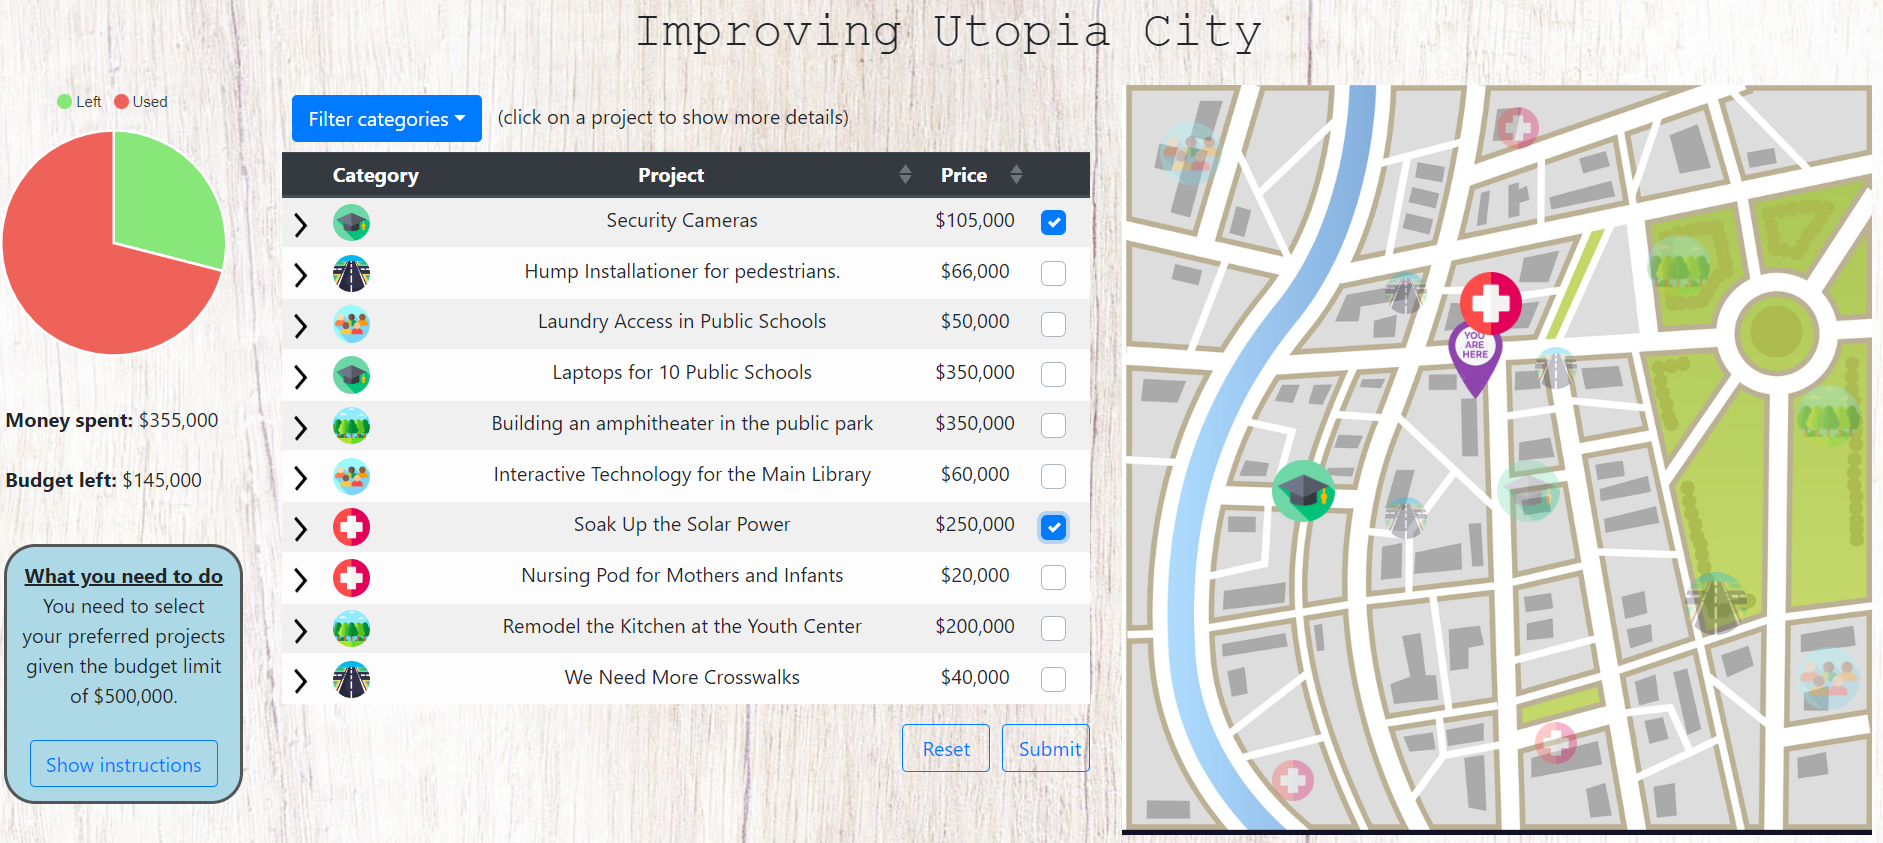
\includegraphics[width=15cm]{experiment/full system.PNG}
\caption{The interface shown to the participants in order to vote.
}\label{fig:interface}
\end{center}
\end{figure}

In Figure~\ref{fig:interface} it possible to see how all of this presented to the participants. In the left side of the screen, they are shown the projects they can choose from and which category it belongs to, and in the right side, there is a map which shows the location of the participant and the location of each of the projects.

Each participant encountered one of the 6 input formats (k approval, threshold approval, knapsack, utilities, ranking by value and ranking by value for money) randomly (the interfaces for them can be seen in Appendix~\ref{app:interfaces}). In addition, the participant is presented with one of four sets of projects, either with 10 projects (noted by elections 3 and 6) or 20 (noted by elections 7 and 8). The exact projects in each election can be seen in Appendix~\ref{app:elections}).

After casting their votes, the participants were presented with  a consistency test with three multiple choice questions 
%(will be referred by consistency test) 
which test whether they understood the task and thought about their choice or just rushed through the task. This way, it is possible to analyze the data only from participants which gave some thought on their response.

Finally, each participant was given a short survey about their experience in the experiment, including six questions: %\gb{...rate on scale of 1 to five the following six..}
\begin{itemize}
    \item \textbf{Ease of use} - We asked participants to rate on a scale of 1 to 5 how easy they found the voting task. %\gb{\textbf{Ease of use} - }how easy they found the voting task.
    \item \textbf{User interface} - We asked participants to rate on a scale of 1 to 5 how much they like the user interface.
    \item \textbf{Perceived expressiveness} - We asked participants to rate on a scale of 1 to 5 how well their vote captured their preferences.
    \item \textbf{Map Accessibility} - We asked the participants to rate on a scale of 1 to 5 how easy was it to access the map.
    \item \textbf{Map effect} - We asked participants to rate on a scale of 1 to 5 how much their and the projects position in the map affected their choice.
    \item \textbf{Categories effect} - We asked participants to rate on a scale of 1 to 5 how much the categories of the projects affected their choice.
\end{itemize}

\section{Aggregation}\label{sec:aggregation}
In this section, we will start the analysis by looking at methods to aggregate the votes in order to choose which projects to fund.
 As mentioned in Section~\ref{sec:intro}, the method that usually used in the real world is greedy aggregation, however, this method have several disadvantages. We will compare it to Rule~X~\citep{peters2020proportional} (RX), showing why it is recommended to use it instead of greedy aggregation. 

Those two methods, based on numeric utility for each of the projects, thus, we will start by explaining how the different formats are represented in utilities. For the approval formats, each approval worth score of 1 and 0 other wise. For the ranking formats, we use Borda score, and finally for utilities the score is the utility given for a project.

In order to compare the two methods, we will use two types of evaluations. First, the outcomes from the aggregation will be compared by the social welfare it achieve for the voters. Second, their stability will be tested, i.e. how well the method can represent the population given only part of it votes.

Starting with welfare, we will first notice that the true utility the voters get from the projects is unknown. Thus, we will use their reported preference and calculate utility as defined above. This mean that for each outcome (from all input formats) we can calculate the social welfare according to 6 different reported votes (one for each input format). 

Figure~\ref{fig:welfare} show the average social welfare (averaged over the four elections) achieved by each of the outcomes according to the knapsack votes. As can be seen, when using the greedy aggregation, the chosen input format have big impact on social welfare, having the outcome from the knapsack votes with highest utility. In contrast, RX achieves almost the same utility, no matter what input format is used, while having social welfare almost as the highest welfare the greedy aggregation achieve. The results following the social welfare of other input formats are similar to those shown in Figure~\ref{fig:welfare}, and can be seen in Appendix~\ref{app:aggregation}.

\begin{figure}[!htbp]
\begin{center}
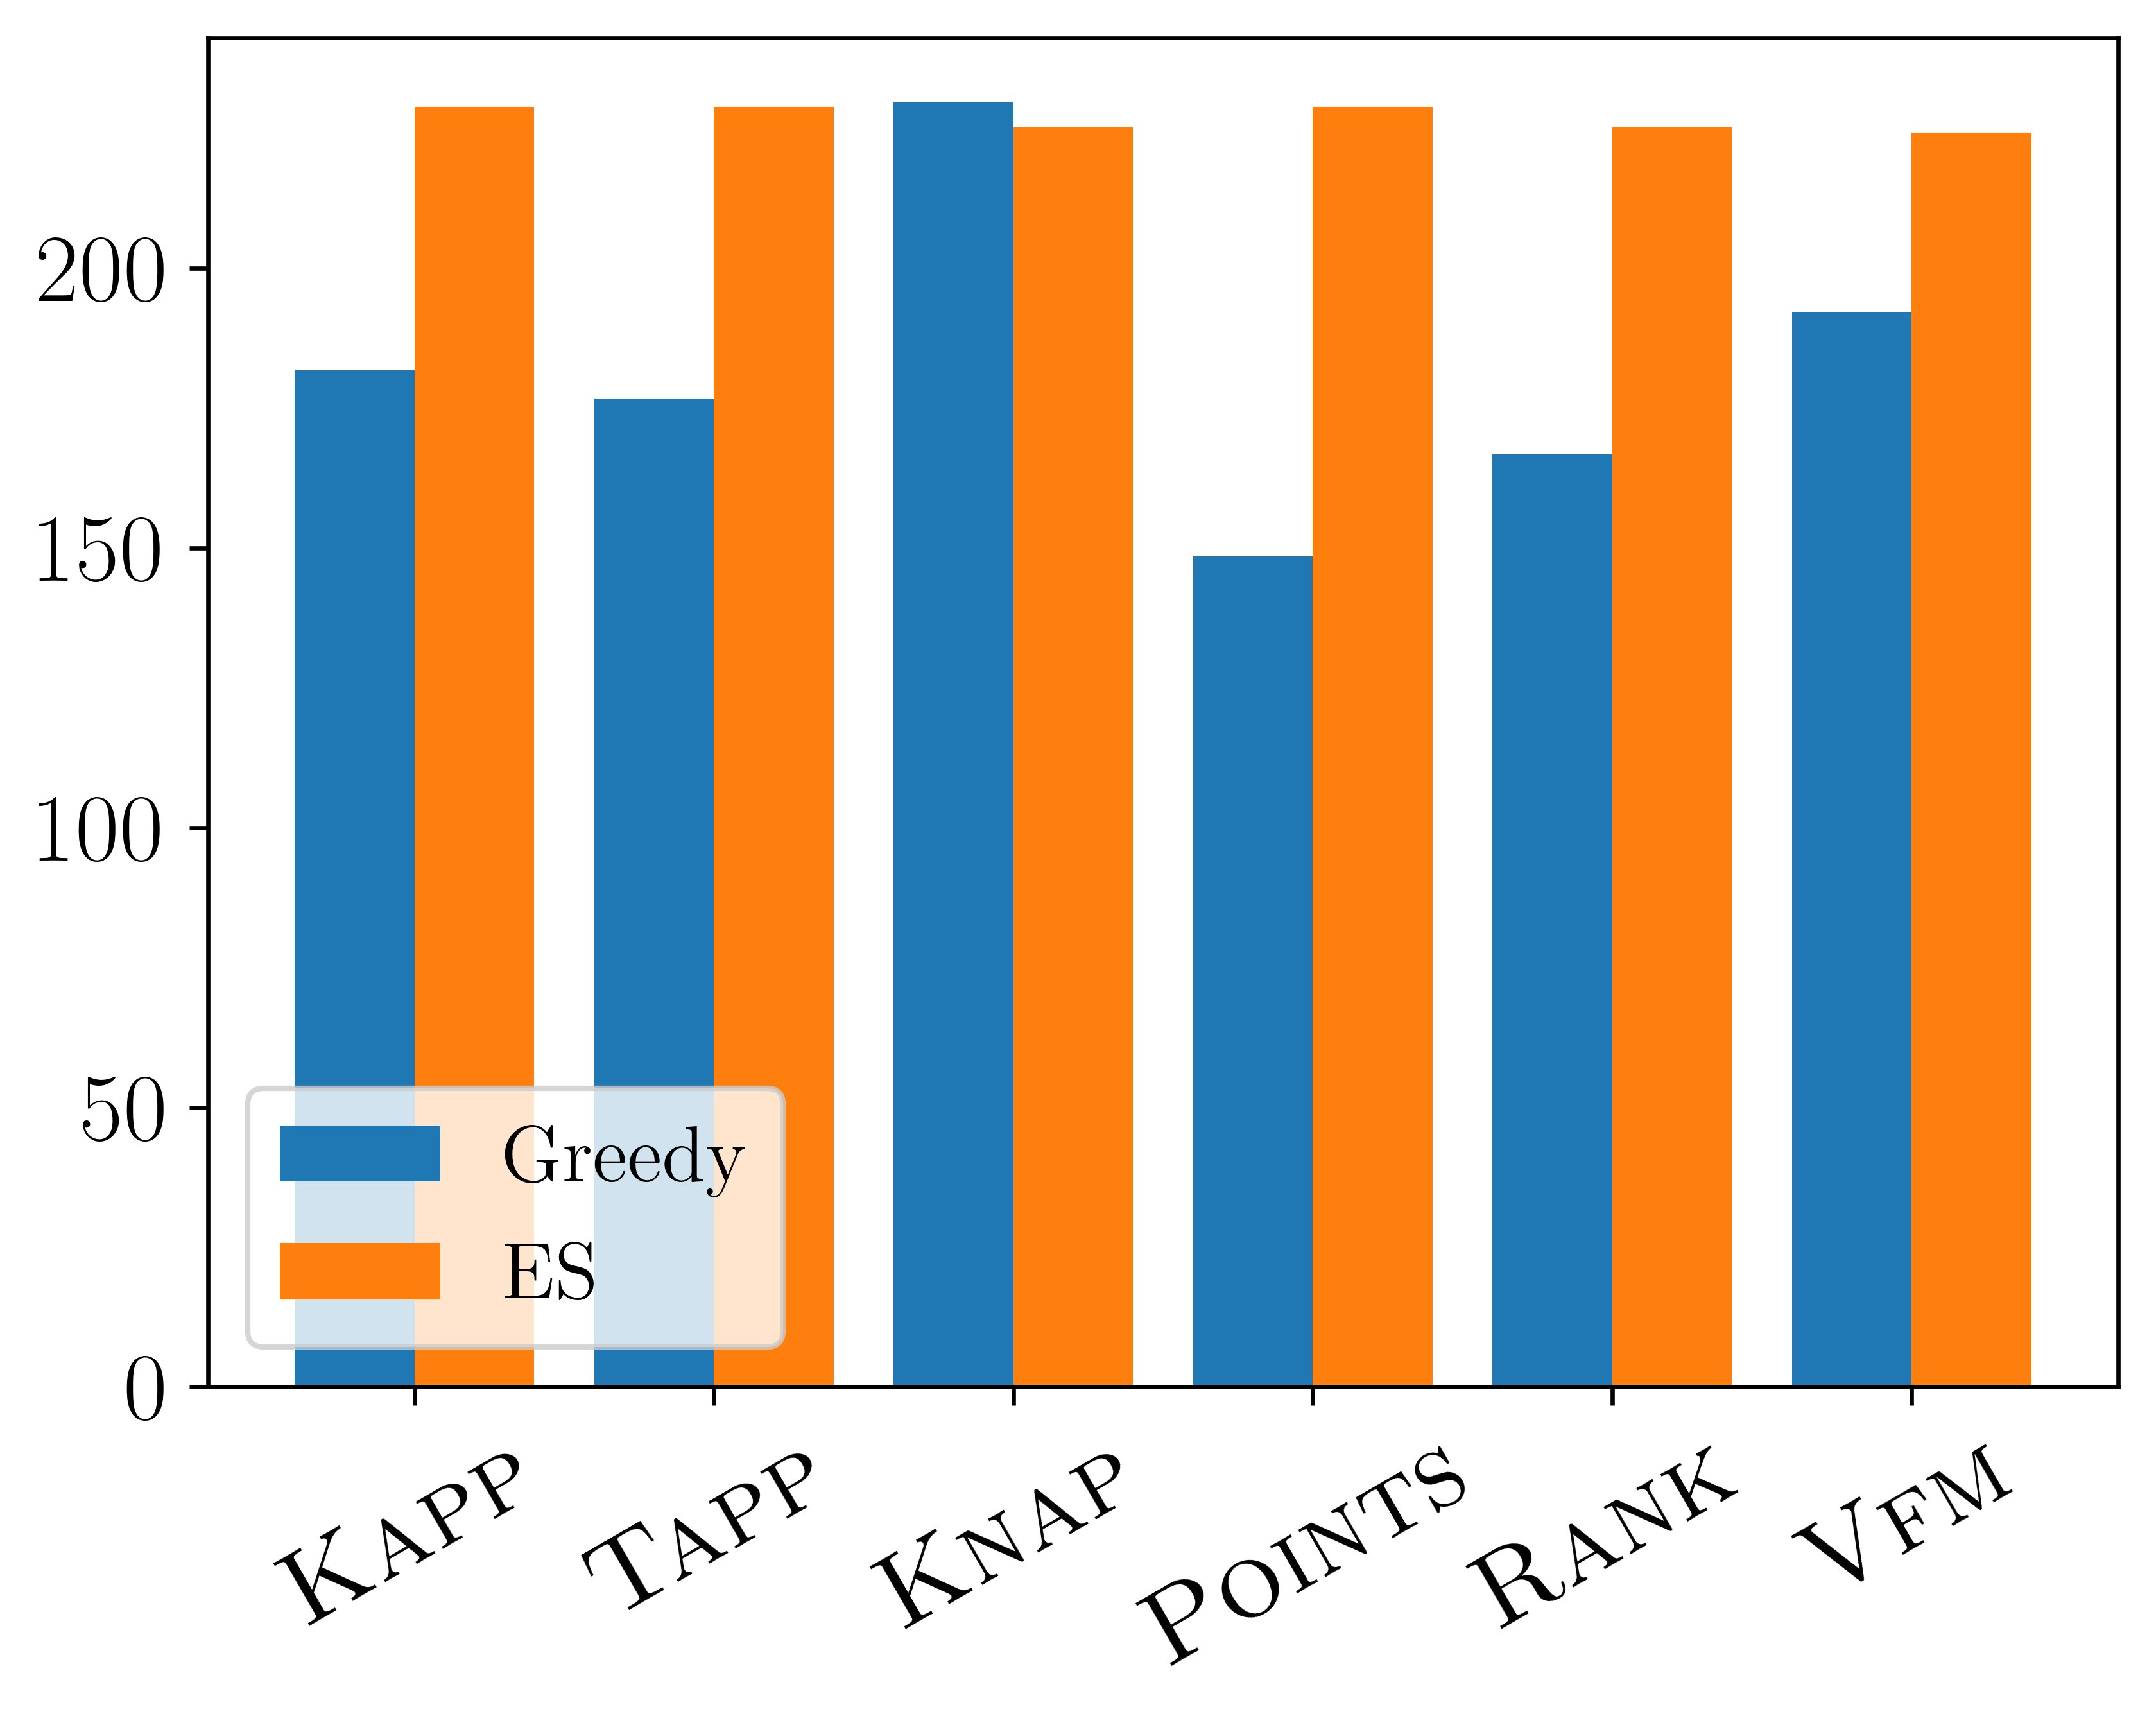
\includegraphics[width=10cm]{experiment/Knapsack_welfare.png}

\caption{Average social welfare for the knapsack voters.
}\label{fig:welfare}
\end{center}
\end{figure}


% Those definitions mean that we have 36 combinations of social welfare per election, six different outcomes and six different social welfare measurement. The results can be seen in Figure~\ref{fig:welfare}, where the welfare was averages over all elections.

% \begin{figure}[!htbp]
% \begin{center}
% 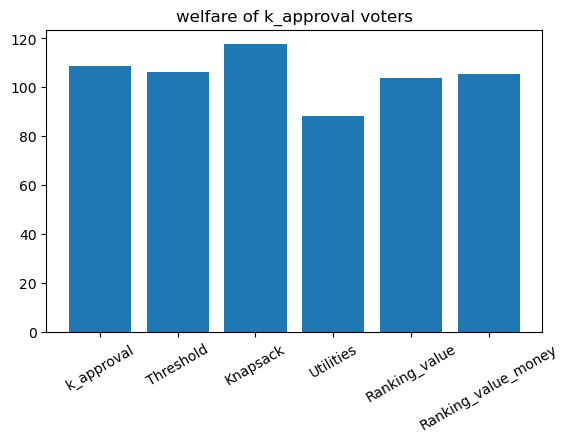
\includegraphics[width=7.5cm]{experiment/welfare_k_approval_avg.png}
% 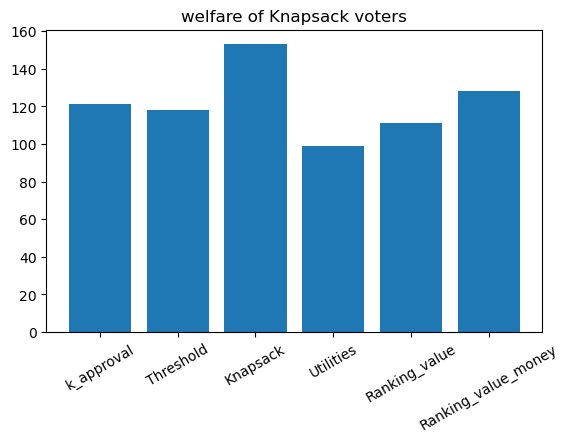
\includegraphics[width=7.5cm]{experiment/welfare_Knapsack_avg.png}
% 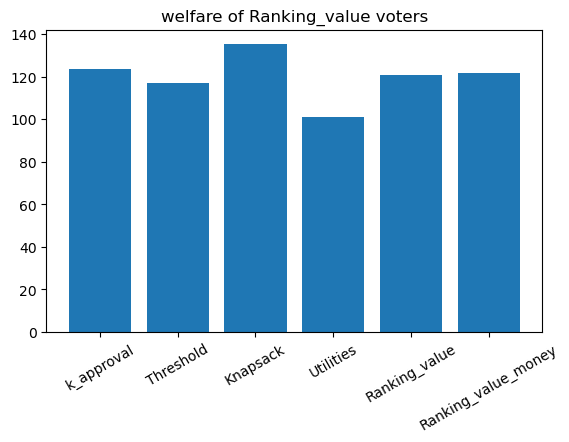
\includegraphics[width=7.5cm]{experiment/welfare_Ranking_value_avg.png}
% 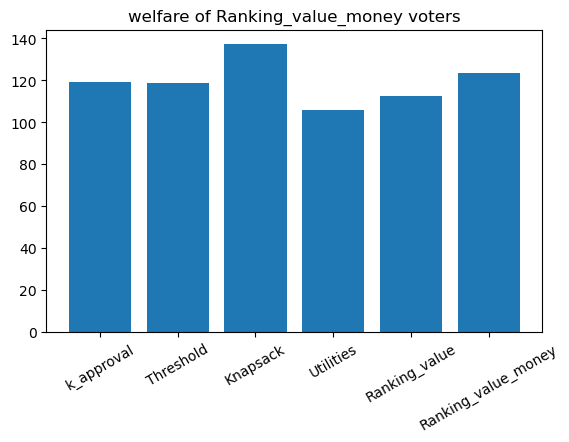
\includegraphics[width=7.5cm]{experiment/welfare_Ranking_value_money_avg.png}
% 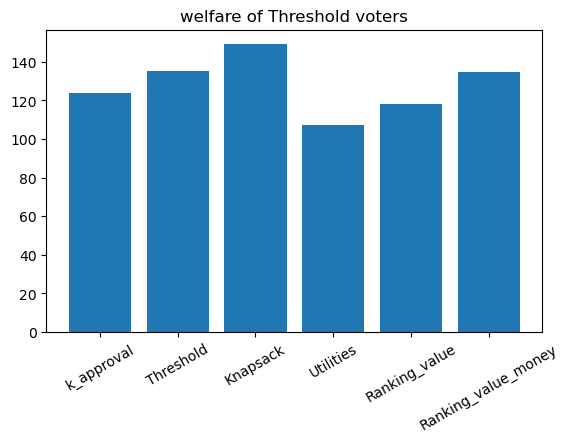
\includegraphics[width=7.5cm]{experiment/welfare_Threshold_avg.png}
% 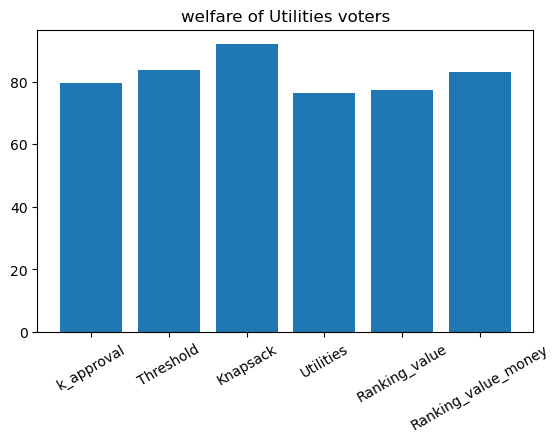
\includegraphics[width=7.5cm]{experiment/welfare_Utilities_avg.png}
% \caption{Average social welfare for each type of input format voters.
% }\label{fig:welfare}
% \end{center}
% \end{figure}

Next, we will look at the stability of the two aggregation methods. To do so, for each election and input format, we will pick uniformly at random a subset of voters and aggregate them to get an outcome. This process is repeated 200 times, counting the percentage of instances where each project was selected. \rf{I want to add here also numeric evaluation to stability to support the claim in addition to the visual results}

The results for election 8 can be seen in the heatmaps in figure~\ref{fig:heatmap}. There are two things that can be inferred from RX heatmap (top):
\begin{enumerate}
    \item Even when different part of the population vote, the outcome stays almost the same.
    \item For all input formats, RX outputs almost the same projects. This also explains the similar welfare across the input formats.
\end{enumerate}

In the greedy heatmap (bottom), we see the exact opposite results from RX. First, the outcome can change a lot, depends on the voters that took part, and therefore, less likely to represent the full population. Second, while there is some similarity in the projects distribution across input formats, there is a dependency between the outcome and the used input format (which supports the results in Figure~\ref{fig:welfare}).

The results for the rest of the elections show similar trends and can be found in Appendix~\ref{app:aggregation}.

\begin{figure}[!htbp]
\begin{center}
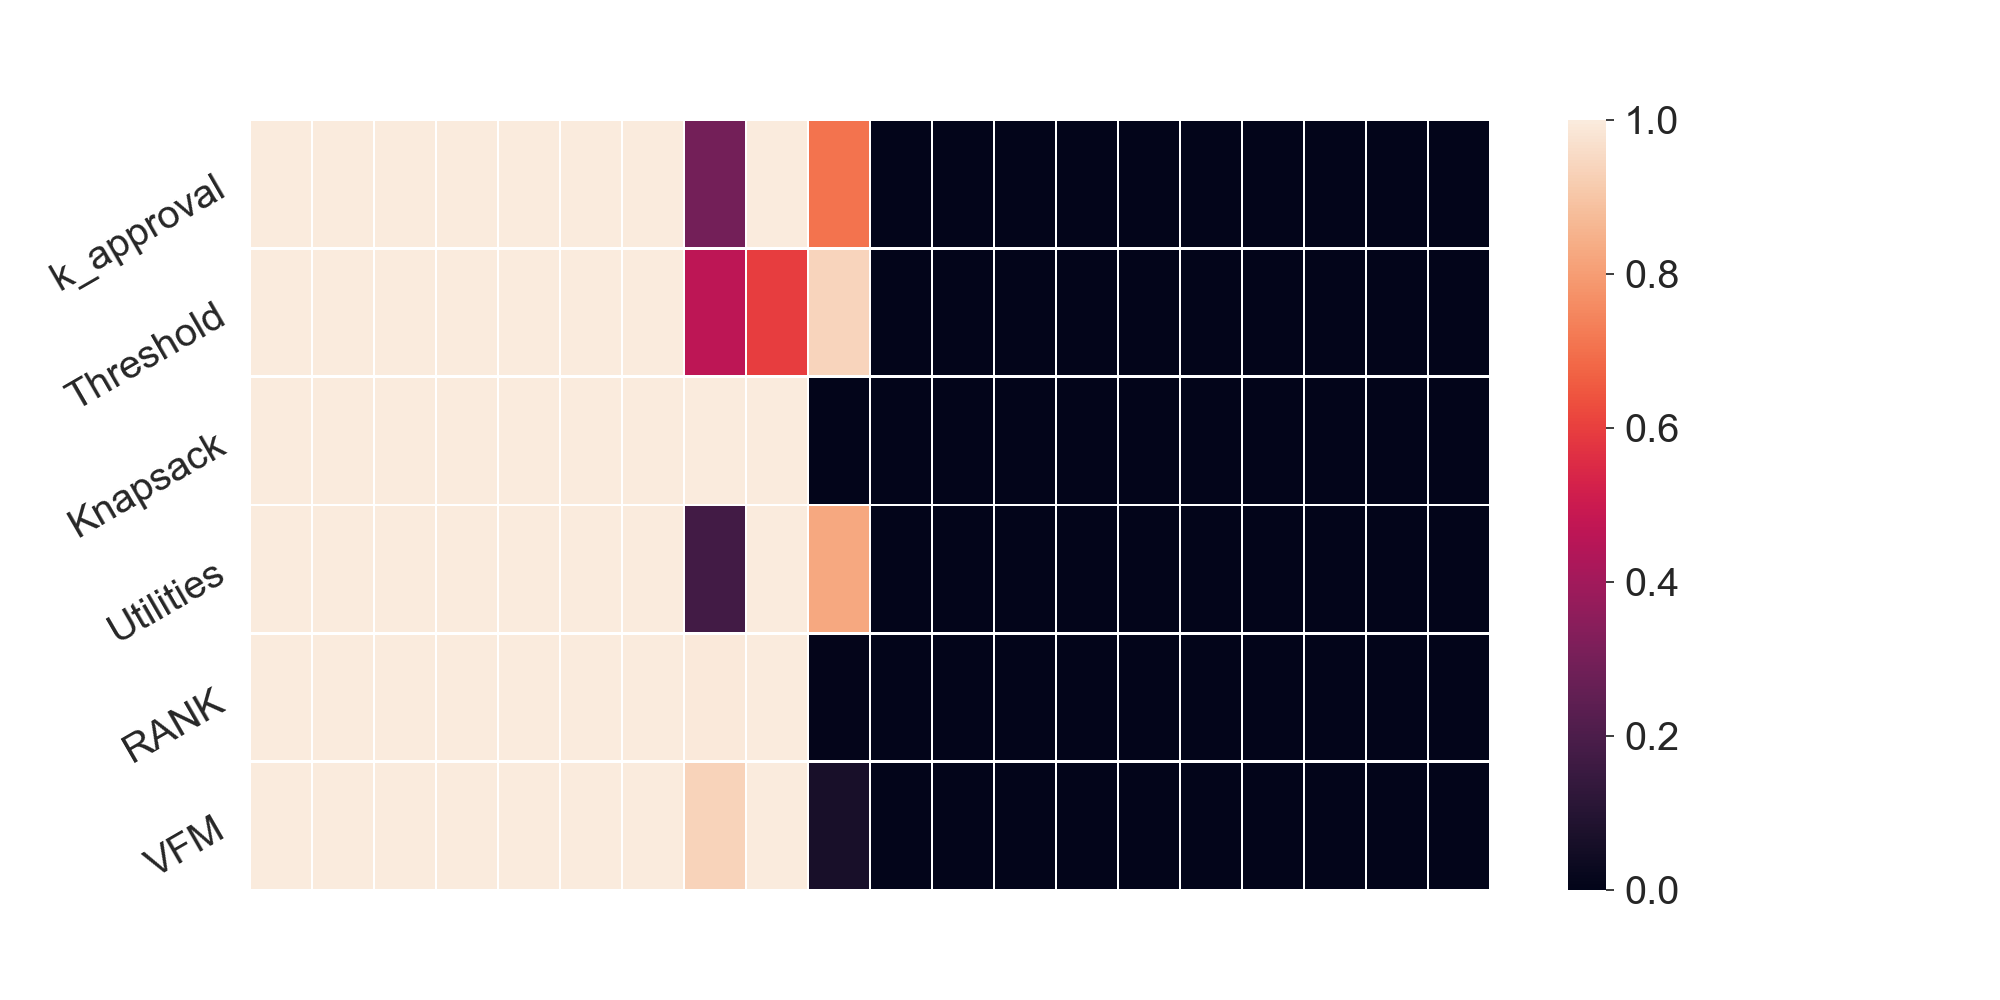
\includegraphics[width=18cm]{experiment/election_8_rx.png}
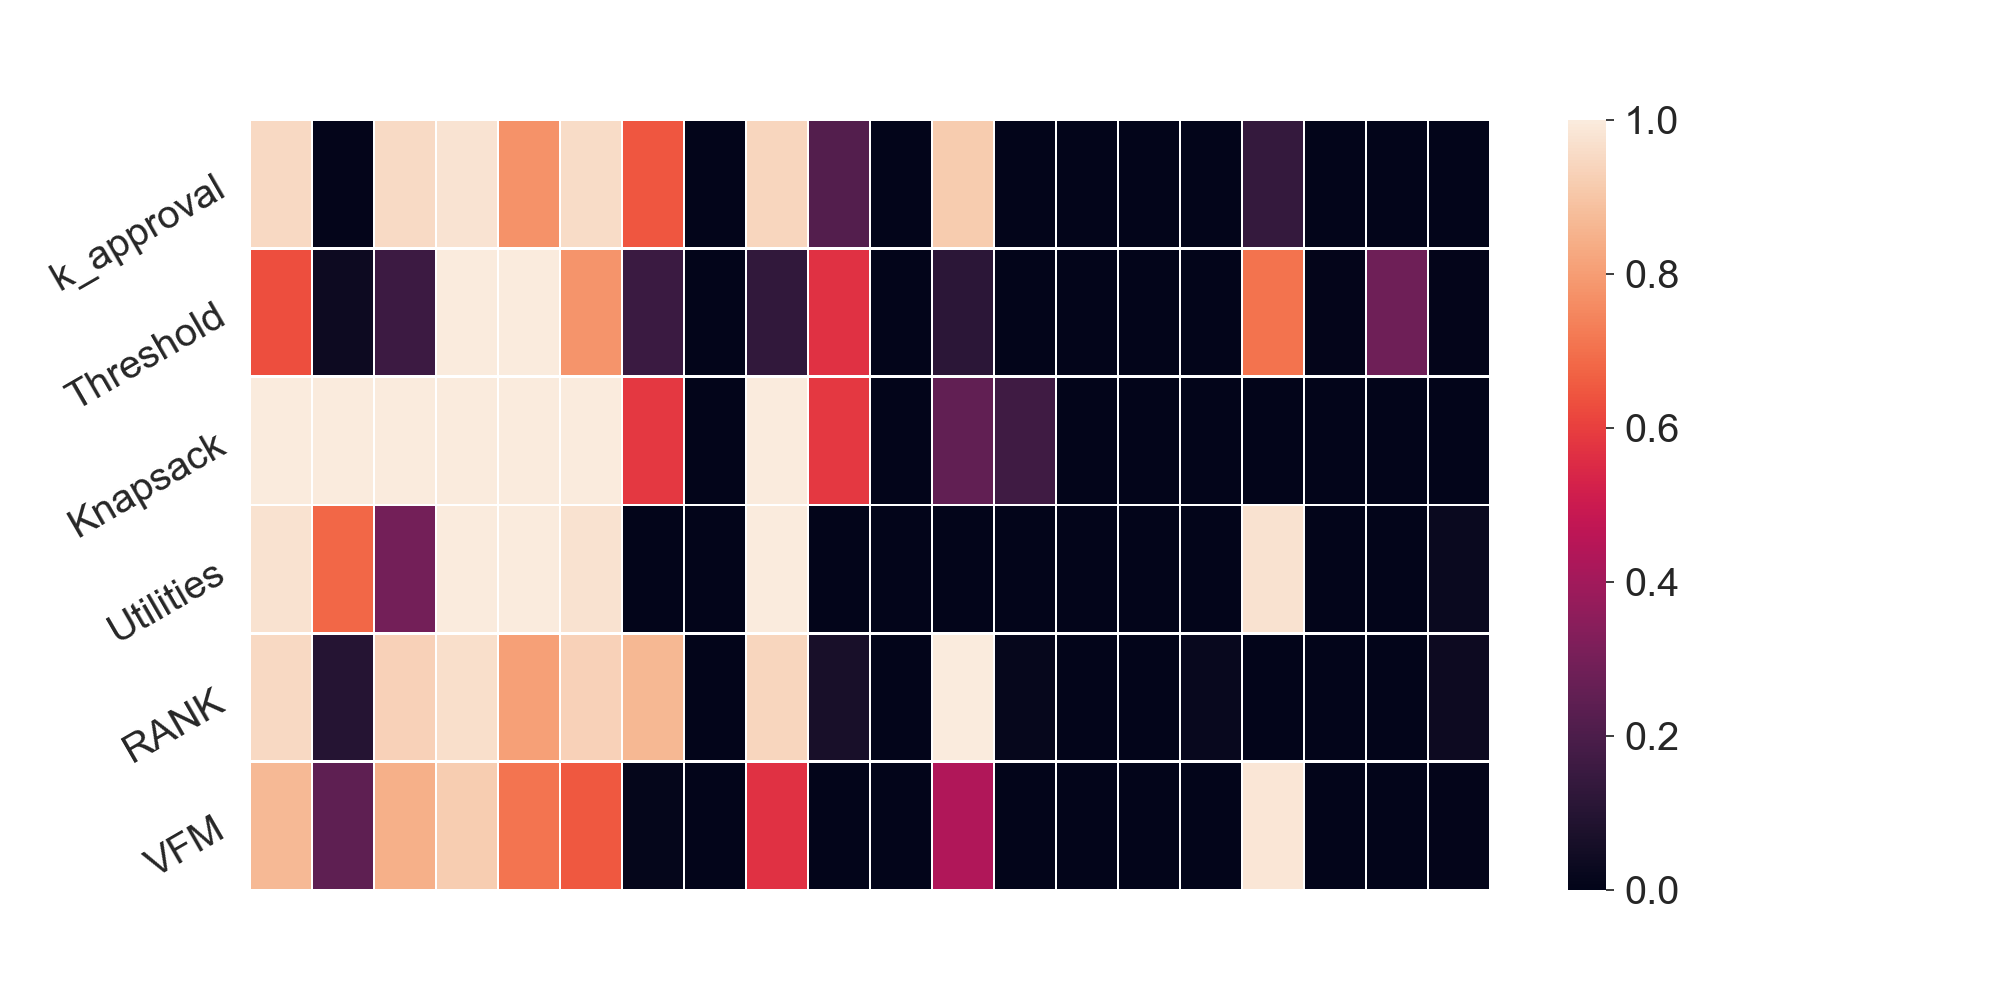
\includegraphics[width=18cm]{experiment/election_8_greedy.png}

\caption{Percentage of instances where each projects was selected for RX (top) and greedy (bottom) aggregation.
}\label{fig:heatmap}
\end{center}
\end{figure}

Finally, we will mention one additional theoretical advantage of RX. It was shown \citep{peters2020proportional} that RX is guaranteed to achieve an proportional outcome, i.e. it ensure  that sufficiently large groups of voters that have similar liked projects must also receive a  fair amount of utility from the outcome. This propriety ensure that minorities who try to promote the same projects will be represented in the outcome. Need to say, that while greedy aggregation can output a proportional outcome, it isn't guaranteed to always do so. 

%%%%%%%%%%%%%%%%%%%%%%%%%%%%%%%%%%%%%%%%%%%%%%%%%%%%%%%
\section{Input Formats}
In this section we will focus on analysing which input format should be used. We will be doing so while keeping in mind the results from the previous section, where we saw than when using RX, the input format used, have very small impact on the outcome, therefore, we will focus on the usability of the input formats. In order to measure this, we look at at objective and subjective indicators, which are inferred from the data collected from the survey the participants submitted.

For the objective indicators we will first look at the results from the consistency test. This test checks how well the participants understood the task they were given, in addition to how much they paid attention and understood what they did in the voting phase.
Second, we record how long it took the participants to do each part in the experiment, which is an indicator on the cognitive burden it created.

As for the subjective indicators, we gave each participant at the end of the experiment a short survey that checks how usable the input format was from their perspective.

\subsection{Objective Indicators}
\emph{\textbf{Consistency.}} We collected 75 participants on average for each of the 24 configurations (6 input formats and 4 projects sets), having 58 participants on average answering the consistency test correctly in each configuration.

From the consistency results, we can infer whether a certain input format or the amount of projects affects on how hard was a configuration to the participants. The results can be seen in Figure~\ref{fig:consistency}.

\begin{figure}[!htbp]
\begin{center}
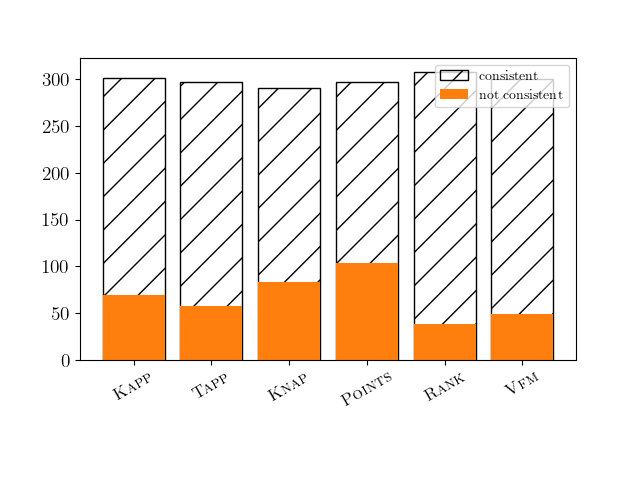
\includegraphics[width=7.5cm]{experiment/format_consistency.png}
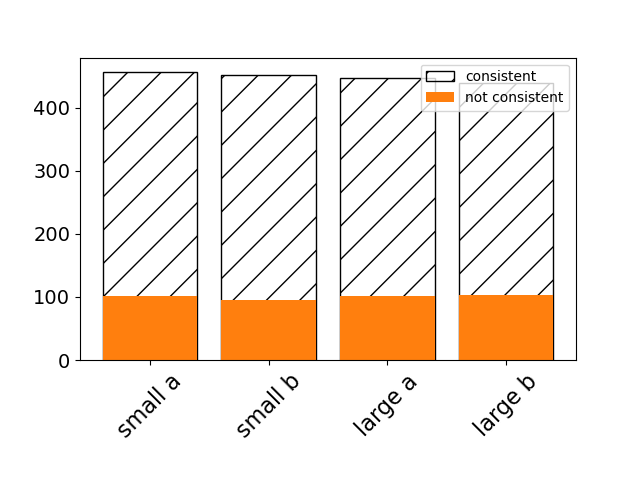
\includegraphics[width=7.5cm]{experiment/election_consistency.png}
\caption{Consistency for each input  format (left) and for each election (right).
%\gb{should label elections properly eventually, not 3,6,etc. }
}\label{fig:consistency}
\end{center}
\end{figure}

As can be seen in Figure~\ref{fig:consistency}, While there is different amount of consistent participants for different input formats, the suggested projects or the number of possible projects have no effect on how consistent participants are. From those results, we can say that participants had the least difficulty in the ranking formats, following by the approval formats and finally the utilities format which as we claimed earlier give the most information, however, take the most cognitive burden on the participant.

\emph{\textbf{Response time.}} 
The time it takes to complete a task is recognized as a good proxy to the cognitive burden it creates \cite{rauterberg1992method}. 
In Figure~\ref{fig:time}, we show for each input format, the average time it took to complete each stage in the experiment.

As can be seen, ranking-value-money takes the longest to learn, to answer the quiz and to cast a vote. This implies on very high cognitive burden this method create, being hard to learn and use.
For the other formats, the learning time and casting time is ranked as follows: K-approval, Knapsack, Ranking-value. Lastly, Threshold was quicker to learn compared to Utilities, but took longer to cast the vote.
%\gb{We should mention/show that the trends are consisitent across elections}


\begin{figure}[!htbp]
\begin{center}
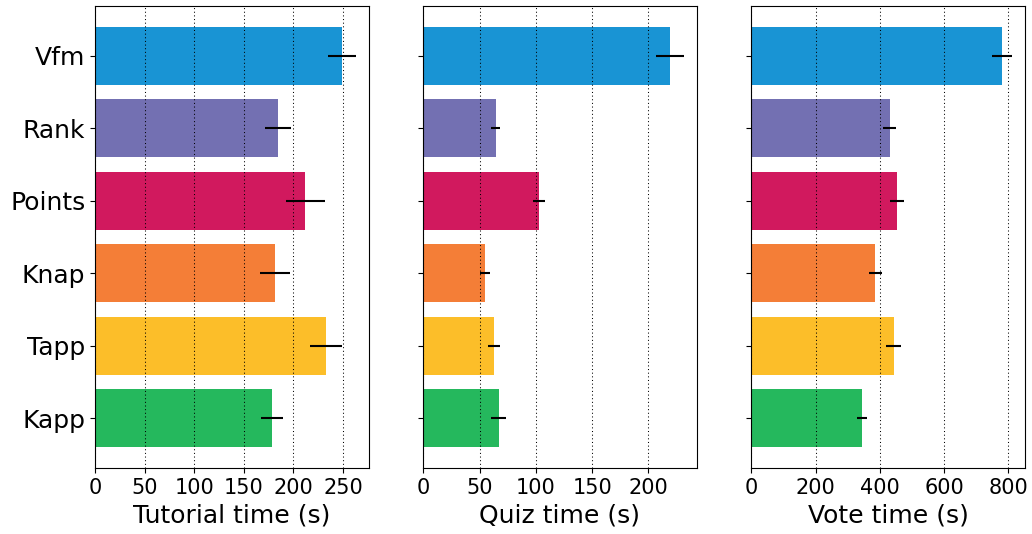
\includegraphics[width=15cm]{experiment/time.png}
\caption{The average time each stage took to the participants.
}\label{fig:time}
\end{center}
\end{figure}

\subsection{Subjective Indicators}
In addition to the objective indicators, we had a survey where we asked the participants about their experience with a certain input format. The result of the survey can be seen at Figure~\ref{fig:feedback}.
When we say below that a result is statistically significant, we are referring to the Mann-Whitney tests at the $p < 0.05$ level. 
%\gb{Is this the best test to run?}


\textbf{Ease of use} - We asked the voters how easy was the voting task. Ranking-value-money is significantly worse than any other input format, while in contrast, k-approval is significantly better than all other input formats except for utilities. 

\textbf{User interface} - We asked the participants how much they liked the interface. Ranking-value-money is significantly worse than any other input format, while in contrast, k-approval is significantly better than all other input formats except for utilities and knapsack.

\textbf{Perceived expressiveness} - We asked the participants how well their vote captured their preferences. The results here are a bit surprising, ranking-value-money is significantly worse than all other formats, even through the same vote is cast as in ranking-value. In addition, we see that k-approval achieve the highest capture (significantly compared to threshold, ranking-value-money and utilities). This is surprising as approval voting let the voter the least power to express themselves, compared to the other formats.


\begin{figure}[!htbp]
\begin{center}
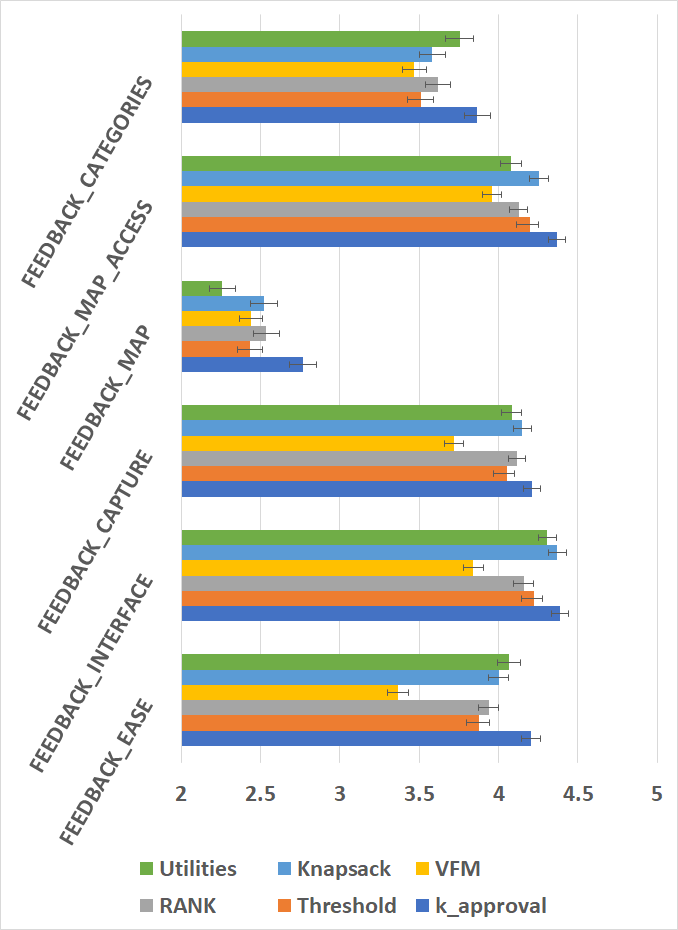
\includegraphics[width=15cm]{experiment/feedback.png}
\caption{The average feedback received for each input format.
}\label{fig:feedback}
\end{center}
\end{figure}

As mentioned in Section~\ref{sec:description}, in order to increase the reality of our experiment, we added location to the voters and projects, in addition to splitting the projects into 5 categories.
In order to check how much we succeeded in this objective, we asked the participants another three questions in the survey: how much the map affected their vote, how much the categories affected their vote and how much accessible was the map.

The results from the two first questions further supports the advantage of using k-approval, which have significantly higher map usage than other formats, and significantly higher categories usage than other formats (except for utilities). This indicates that low cognitive burden caused from using k-approval, enable the voters to take into consideration other factors that might be important for them, and not only the project description.

Finally, we can see that the map usage is quite low, which the last question come to check if it caused by inaccessibility of the participants to the map. From the results it possible to see that the interface made the map accessible enough, and the participants give the location less significance compared to other factors.


\section{Discussion}
Our results shed light on the advantages and disadvantages of different input formats using objective and subjective indicators in the voting stage, in addition to comparison in social welfare achieved by the different formats.

From those tests we get that k-approval have the lead in the subjective indicators and in the response time, making it a clear winner when looking for usability and lowering the voters cognitive burden. In contrast, even through it is clear what the task is with ranking-value-money (high consistency), participants had hard time with this format, suggesting very low usability.

Next, we tested two aggregation method (greedy and RX), and showed the advantages of using RX over greedy. First, RX is much more stable, i.e. it is likely for the outcome to stay almost the same, even if only part of the population votes. This is very important when talking about PB as in many cases the participation is quite low. For example, \citet{zepic2017participatory} talks about a case in Germany where only 0.1\% of the eligible voters actually voted. 

Second, RX outputs almost the same outcome no matter what input format is used. This result is extremely important, as it let the organizers to choose whatever input format they like to without having significant impact on the outcome.

This can be concluded to a strong recommendation for PB organizers to switch from using greedy aggregation to RX. In doing so, we can recommend in a full heart to keep using k-approval as been done so far, since using it will have small impact on the outcome, while being subjectively the favorite format, thus lowering the frustration of the voters when taking part, making it more likely that will participate again,

% It is also important to notice knapsack, which isn't the best in terms of usability, however, is not far behind k-approval. This is in addition to achieving the highest social welfare, making it a good candidate as an input format. Those results corroborate the results of \cite{goel2016knapsack, goel2019knapsack}.

% Finally, looking at the utility input format. The results are consistent with Section~\ref{sec:intro} which says it cause the voter high cognitive burden. While the participants reported it was easy to use, it had the highest inconsistency, meaning they had harder time to use this input format causing their vote being less representative. This in turn make the outcome worse for the population, achieving the lowest social welfare.

Finally, we discuss several limitations of our study, and points to future work. While trying to mimic as most as possible a scenario of real world participatory budgeting, there still is place for improvements, such as increasing the value of the location, for example, giving more details on the city size, and suggesting projects that might have more effect according to their proximity to your house.

Next, our experiment included a single vote, receiving no feedback on the outcome. This raise the need for a continuation experiment which will add another level of subjective indication on the outcome of specific input format. First, it possible to add another stage to the experiment, where they are asked to rank how satisfied from the outcome (using previous data to create it). In addition, to create a completely objective experiment (without any attachments), it is possible to give the participants information about the city in addition to the votes, and showing several outcomes from different input formats, asking the participants to choose which is better for the general population in terms of social welfare and are minorities represented enough?

%%%%%%%%%%%%%%%%%%%%%%%%%%%%%%%%%%%%%%%%%
\bibliographystyle{plainnat}
\bibliography{ref.bib}


%%%%%%%%%%%%%%%%%%%%%%%%%%%%%%%%%%%%%

\begin{appendices}

\section{Interface For Voting}\label{app:interfaces}
Table~\ref{tab:all_interfaces} show what the interface to vote look like for each of the input formats.

\begin{table}[ht!]
  \begin{center}
    \begin{tabular}{|c|c|}
    \hline
    \makecell{K approval \\ 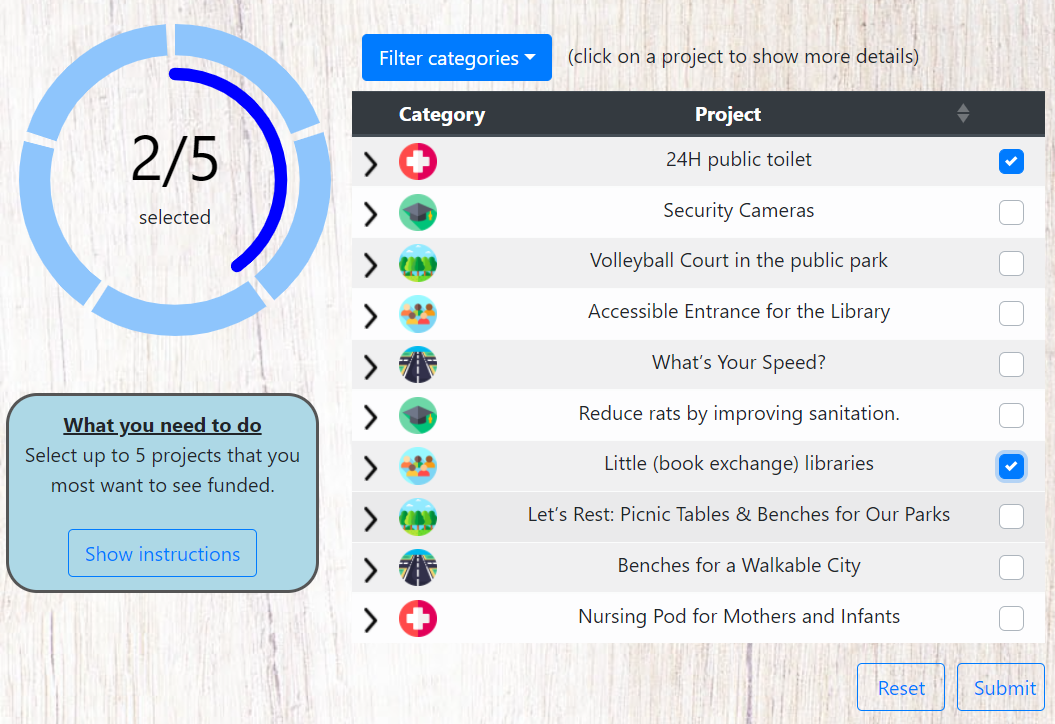
\includegraphics[width=7.5cm]{experiment/k approval.PNG}} & \makecell{Threshold approval \\  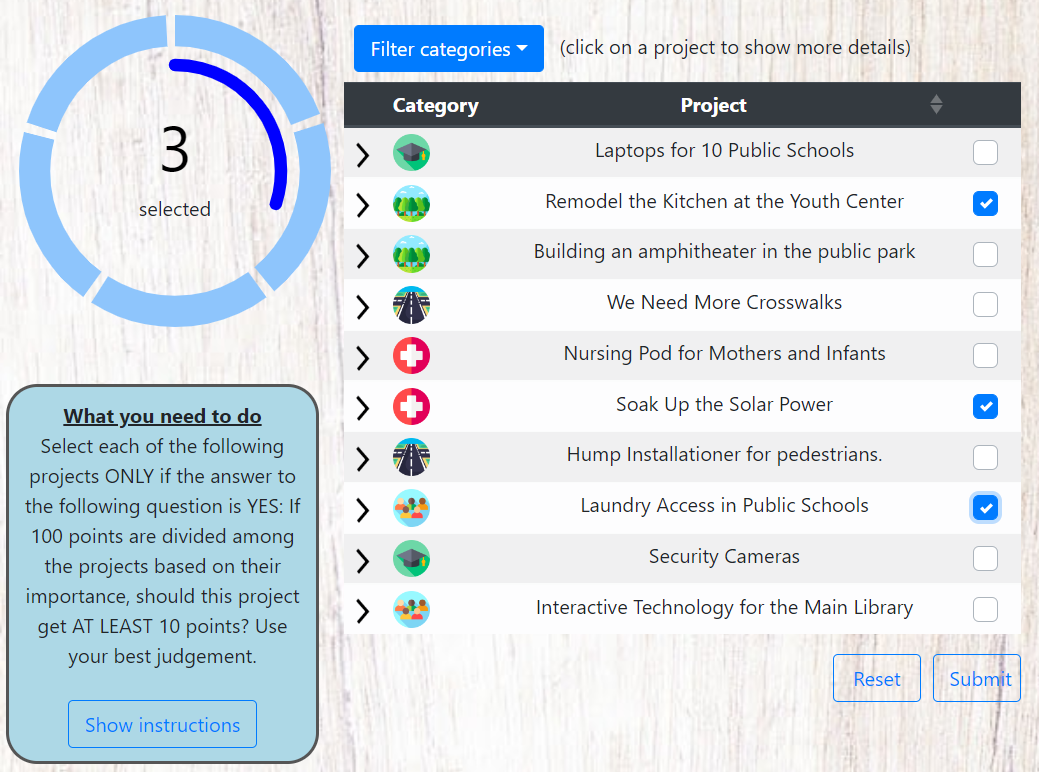
\includegraphics[width=7.5cm]{experiment/threshold approval.PNG}}\\
    \hline
    \makecell{Knapsack \\ 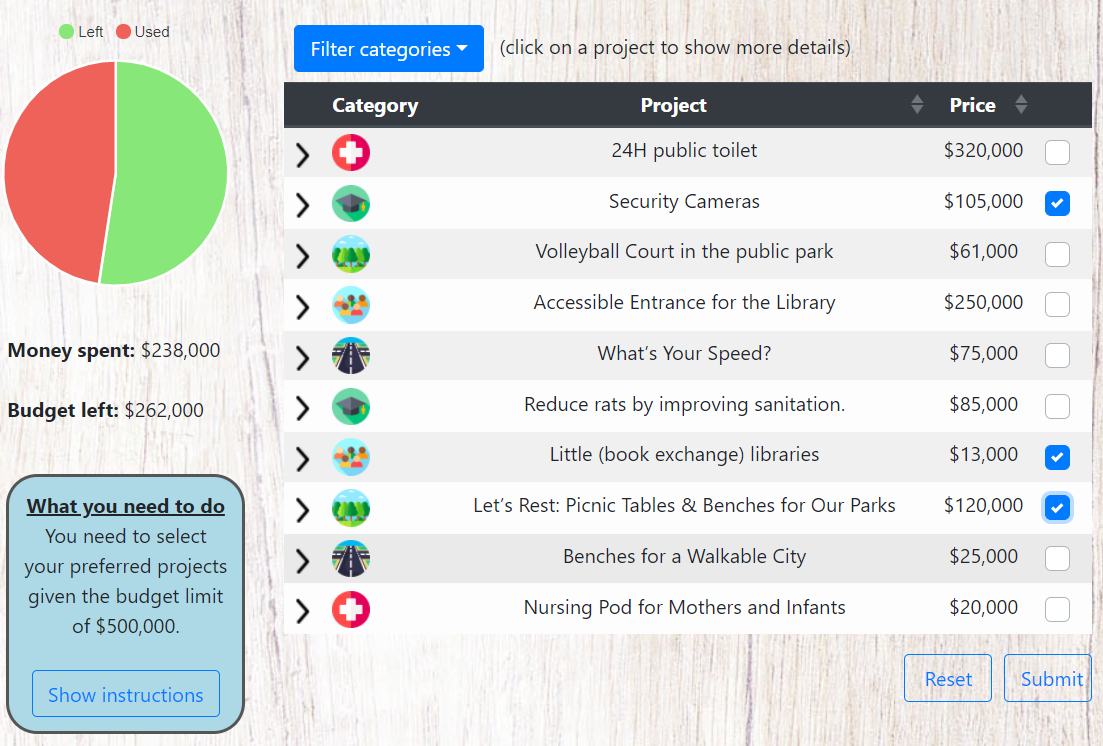
\includegraphics[width=7.5cm]{experiment/knapsack.PNG}} & 
    \makecell{Utilities \\ 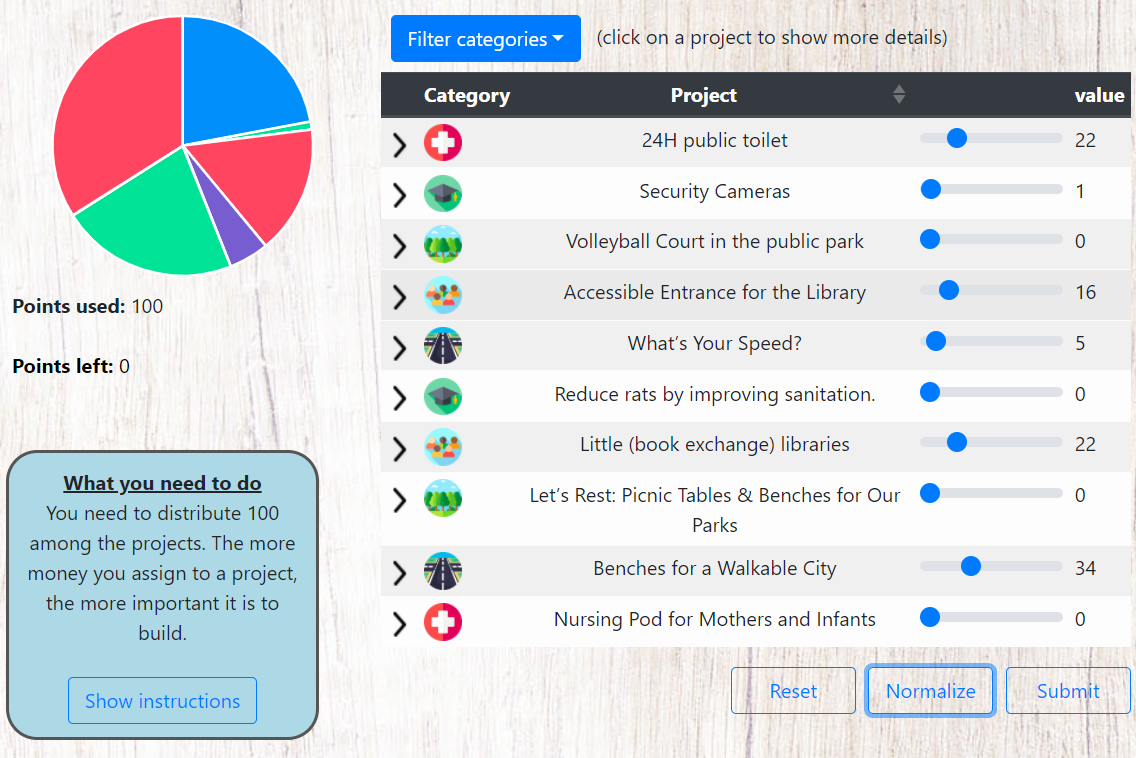
\includegraphics[width=7.5cm]{experiment/utilities.PNG}}\\
    \hline
    \makecell{Ranking by value \\ 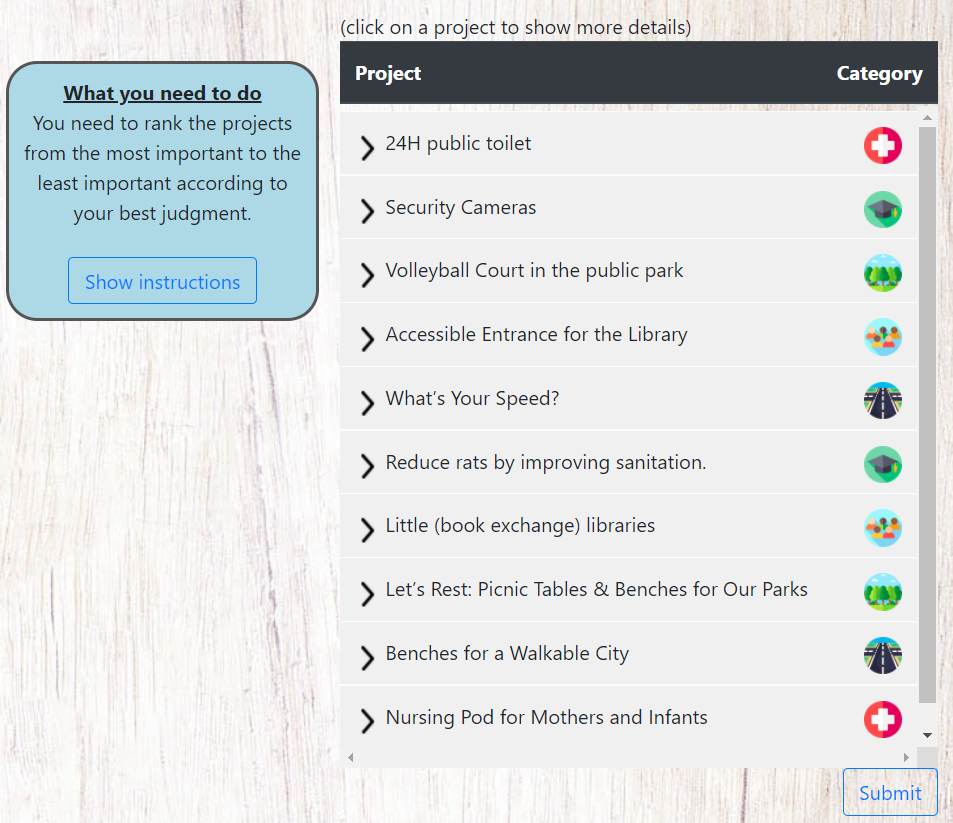
\includegraphics[width=7cm]{experiment/ranking.PNG}} &
    \makecell{Ranking by value for money \\ 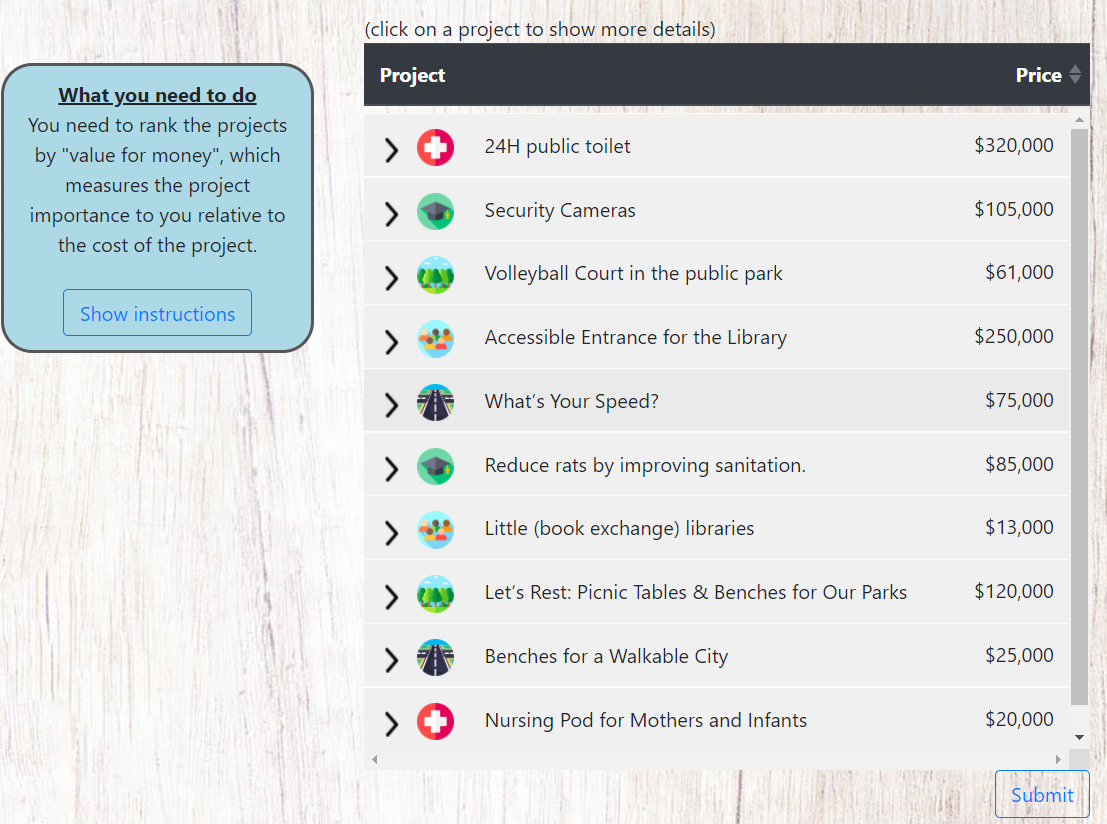
\includegraphics[width=7.5cm]{experiment/ranking by cost.PNG}}\\

        
     \hline
    \end{tabular}
  \caption{Input formats interface}\label{tab:all_interfaces}.
  \end{center}
\end{table}

\section{Experiment Configurations}\label{app:elections}

In the experiments each participant encountered one of six input formats and one of 4 possible elections, each with different set of projects, either 10 projects or 20, such that each project belong to one of 5 categories:

\begin{itemize}
    \item Culture and community.
    \item Streets, Sidewalks and Transit.
    \item Environment, public health and safety.
    \item Facilities, parks and recreation.
    \item Education.
\end{itemize}

Tables~\ref{tab:first_elc}-\ref{tab:fourth_elc} show the four different elections the participants might encounter in the experiment, a short description, and to which category it belongs.

\begin{table}[ht!]
  \begin{center}
    \begin{tabular}{|p{4cm}|p{8cm}|p{3cm}|c|}
    \hline
    \textbf{Project} & \textbf{Description} & \textbf{Category} & \textbf{Price}\\
    \hline
    Computers for the community learning center & Funding 20 laptops including mice and keyboards, giving students a place to study & Culture and community &  27K\\
    \hline
    Laundry Access in Public Schools & Renovate a space in a Cambridge Public School and install washers and dryers for students who do not have easy access to laundry services at home, to use for their clothing and necessities & Culture and community & 50K\\
    \hline
    Real-Time Bus Arrival Monitors in bus stations & Real-time bus arrival monitors bus stops will inform travelers when the next bus will arrive, so they can adjust their plans if needed &  Streets, Sidewalks and Transit &  24K\\
    \hline
    Sheltered Bike Parking at the Main Library & The Main Library needs more bicycle parking. A glass pavilion, protecting bikes from the weather, landscaped with paths and trees, will be an attractive and functional addition to the library grounds & Streets, Sidewalks and Transit & 90K\\
    \hline
    24H public toilet & 24-hour access public toilet near Central Square & Environment, public health and safety & 320K\\
    \hline
    The Sustainable Energy Pilot & Install energy conversion devices on gym equipment and a rapid electric vehicle charging station & Environment, public health and safety & 90K\\
    \hline
    Dog Park & Building a dog park & Facilities, parks and recreation & 250K\\
    \hline
    Let’s Rest: Picnic Tables and Benches for Our Parks & Benches and picnic tables bring our community together. Installing new benches and picnic tables in up to 10 of our park will allow people of all ages and abilities to enjoy them for resting, talking, reading, people watching and being outdoors & Facilities, parks and recreation & 120K\\
    \hline
    Installing Lights at the school Basketball Court & Install lighting to extend safe playing hours for basketball courts. Increases safety for community members while expanding healthy alternatives for youth and access to public space & Education & 250K\\
    \hline
    Security Cameras & Install security cameras in public schools & Education & 105K\\
        
     \hline
    \end{tabular}
  \caption{First small election}\label{tab:first_elc}.
  \end{center}
\end{table}

\begin{table}[ht!]
  \begin{center}
    \begin{tabular}{|p{4cm}|p{8cm}|p{3cm}|c|}
    \hline
    \textbf{Project} & \textbf{Description} & \textbf{Category} & \textbf{Price}\\
    \hline
    Interactive Technology for the Main Library & This project will fund an iPad lending kiosk and 16 iPads, as well as a permanent interactive screen in the Children’s Room of the Main Library & Culture and community & 60K\\
    \hline
    Laundry Access in Public Schools & Renovate a space in a Cambridge Public School and install washers and dryers for students who do not have easy access to laundry services at home, to use for their clothing and necessities & Culture and community & 50K\\
    \hline
    We Need More Crosswalks & To enhance pedestrian safety, this project will add a minimum of five new crosswalks to major streets & Streets, Sidewalks and Transit &  40K\\
    \hline
    Hump Installationer for pedestrians & Speed humps create a safer environment by helping slow traffic on streets that students and families cross frequently. When a car hits a pedestrian at a high rate of speed, the collision is more likely to result in a pedestrian fatality. Speed humps slow vehicles and give drivers increased response time and distance for stopping. This makes streets safer for pedestrians & Streets, Sidewalks and Transit & 66K\\
    \hline
    Nursing Pod for Mothers and Infants & Provide an attractive private space where working mothers and community members can breastfeed or pump during the work day & Environment, public health and safety & 20K\\
    \hline
    Soak Up the Solar Power & Free, clean, renewable energy! Let’s add solar panels to the Youth Center to reduce greenhouse gas emissions and save money on energy & Environment, public health and safety & 250K\\
    \hline
    Building an amphitheater in the public park & Build an amphitheater in the public park for outdoor performances, music, stories, and other cultural events that the whole community can enjoy & Facilities, parks and recreation & 350K\\
    \hline
    Remodel the Kitchen at the Youth Center & The kitchen area in the Youth Center is in dire need of renovating. Replace the stove, dishwasher, cabinets, and countertops in the Youth Center kitchen & Facilities, parks and recreation & 200K\\
    \hline
    Laptops for 10 Public Schools & Purchasing laptop carts for ten public schools & Education & 350K\\
    \hline
    Security Cameras & Install security cameras in public schools & Education & 105K\\
     \hline
    \end{tabular}
  \caption{Second small election}\label{tab:second_elc}.
  \end{center}
\end{table}

\begin{longtable}[ht!]{|p{4cm}|p{8cm}|p{3cm}|c|}
    \hline
    \textbf{Project} & \textbf{Description} & \textbf{Category} & \textbf{Price}\\
    \hline
    Little (book exchange) libraries &  Installing 13 little free libraries across town & Culture and community & 13K\\
    \hline
    Computers for the community learning center & Funding 20 laptops including mice and keyboards, giving students a place to study & Culture and community &  27K\\
    \hline
    Digital Sign at City Hall in Multiple Languages & Digital sign that will scroll announcements in multiple languages and welcome people to town & Culture and community & 75K\\
    \hline
    Meeting Room Upgrade for libraries & Upgrades will allow for the latest in technology be available for public use in the meeting room & Culture and community &  250K\\
    \hline
    Separate Bike Lanes from Traffic & Improve safety for drivers and bikers by moving bike lanes to be between street parking spots and the sidewalk, reducing car-bike interactions and potential collisions & Streets, Sidewalks and Transit & 50K\\
    \hline
    Real-Time Bus Arrival Monitors in bus stations & Real-time bus arrival monitors bus stops will inform travelers when the next bus will arrive, so they can adjust their plans if needed &  Streets, Sidewalks and Transit &  24K\\
    \hline
    Benches for a Walkable City & Install 12 benches across town so that people of all ages and abilities can enjoy benches for resting, talking, tinkering with electronic devices, people watching, and being outdoors & Streets, Sidewalks and Transit & 25K\\
    \hline
    Urban Bicycle Wash Stations & Bicycle owners need to clean and care for their bikes, ideally monthly. But for apartment dwellers, this is really hard! These centrally located bicycle wash stations would allow bicycle owners to wash off dirt, grime, and salt from their bikes & Streets, Sidewalks and Transit & 20K\\
    \hline
    Planting trees in the city & Street trees cool the city, absorb pollution, and make our neighborhoods more livable! planting 100 new trees and building tree wells in the areas that need them most & Environment, public health and safety & 119.4K\\
    \hline
    24H public toilet & 24-hour access public toilet near Central Square & Environment, public health and safety & 320K\\
    \hline
    5 Water Bottle Refill Stations & At a water bottle refill station you get a healthy drink for free & Environment, public health and safety & 40K\\
    \hline
    Fire Hydrant Markers & Install high-visibility markers on fire hydrants around town to increase safety for all residents and reduce response time of the fire department by improving ease of locating hydrants in emergencies, at night, and in the snow & Environment, public health and safety & 8K\\
    \hline
    Outdoor Fitness Equipment in the public park & Install outdoor body-weight fitness equipment for stretching, strength building, and plyometric exercises & Facilities, parks and recreation & 65K\\
    \hline
    Volleyball Court in the public park & Creating an outdoor volleyball court would be an exciting addition to the city. The court would have sand and a sturdy net for three-season usage & Facilities, parks and recreation & 61K\\
    \hline
    Inclusive Playground for All Kids & This Universal Design playground would include equipment that is designed to be usable by everyone without special adaptations or retrofitting & Facilities, parks and recreation & 305K\\
    \hline
    Protect the Health and Safety of our Firefighters & This proposal will purchase and install six gear drying units to shorten wait time for clean gear (\$55,000), and eleven sets of wireless headsets to protect hearing and improve communication (\$55,000). Let’s protect those who protect us & Facilities, parks and recreation & 110K\\
    \hline
    New Chairs for Public Schools & New Chairs for Public Schools & Education & 190K\\
    \hline
    Invention and Production of Music & Install music studios and equipment at the Youth Centers to inspire creativity, enable pre-teens and teens to express their skills and passions, and provide youth with another recreational outlet & Education & 150K\\
    \hline
    Upgraded Water Fountains for Public Schools & Project would install 35 new water bottle refilling fountains in public schools & Education & 200K\\
    \hline
    New Playground for public school & Playground should include a jungle gym, and other equipment for kids to play different games & Education & 200K\\

     \hline
    % \end{tabular}
  \caption{First big election}\label{tab:third_elc}.
%   \end{center}
\end{longtable}

\begin{longtable}[ht!]{|p{4cm}|p{8cm}|p{3cm}|c|}
%   \begin{center}
    % \begin{tabular}{|p{4cm}|p{8cm}|p{3cm}|c|}
    \hline
    \textbf{Project} & \textbf{Description} & \textbf{Category} & \textbf{Price}\\
    \hline
    Little (book exchange) libraries &  Installing 13 little free libraries across town & Culture and community & 13K\\
    \hline
    Computers for the community learning center & Funding 20 laptops including mice and keyboards, giving students a place to study & Culture and community &  27K\\
    \hline
    Meeting Room Upgrade for libraries & Upgrades will allow for the latest in technology be available for public use in the meeting room & Culture and community &  250K\\
    \hline
    Accessible Entrance for the Library & Add automatic sliding doors, fix driveway and, if needed, remove steps to benefit seniors and people with disabilities & Culture and community & 250K\\
    \hline
    Bike repair stations & Install 8 bike repair stations with tools and bike pumps across the city for cyclists to quickly, easily, and freely fix routine bike problems & Streets, Sidewalks and Transit & 12K\\
    \hline
    Separate Bike Lanes from Traffic & Improve safety for drivers and bikers by moving bike lanes to be between street parking spots and the sidewalk, reducing car-bike interactions and potential collisions & Streets, Sidewalks and Transit & 50K\\
    \hline
    Sheltered Bike Parking at the Main Library & The Main Library needs more bicycle parking. A glass pavilion, protecting bikes from the weather, landscaped with paths and trees, will be an attractive and functional addition to the library grounds & Streets, Sidewalks and Transit & 90K\\
    \hline
    What’s Your Speed? & Remind drivers to slow down by deploying live speed displays on busiest streets &  Streets, Sidewalks and Transit & 75K\\
    \hline
    24H public toilet & 24-hour access public toilet near Central Square & Environment, public health and safety & 320K\\
    \hline
    Flashing Crosswalks for Safer Streets & This project would fund rapid flashing beacons at 10 high pedestrian risk crosswalks. These beacons increase the visibility of pedestrians, especially at night. They can alert drivers to crossing pedestrians, thereby preventing crashes & Environment, public health and safety & 176K\\
    \hline
    Soak Up the Solar Power & Free, clean, renewable energy! Let’s add solar panels to the Youth Center to reduce greenhouse gas emissions and save money on energy & Environment, public health and safety & 250K\\
    \hline
    Fire Hydrant Markers & Install high-visibility markers on fire hydrants around town to increase safety for all residents and reduce response time of the fire department by improving ease of locating hydrants in emergencies, at night, and in the snow & Environment, public health and safety & 8K\\
    \hline
    Free Wifi in 6 Outdoor Public Spaces & Install special outdoor wifi access points to offer free public wifi in the public space & Facilities, parks and recreation & 42K\\
    \hline
    Inclusive Playground for All Kids & This Universal Design playground would include equipment that is designed to be usable by everyone without special adaptations or retrofitting & Facilities, parks and recreation & 305K\\
    \hline
    Shade and Wet Weather Canopies for Playgrounds & Installing canopies over playgrounds that do not have protection from the elements will reduce weather-related safety concerns and increase playground availability and use & Facilities, parks and recreation & 146K\\
    \hline
    Let’s Rest: Picnic Tables and Benches for Our Parks & Benches and picnic tables bring our community together. Installing new benches and picnic tables in up to 10 of our park will allow people of all ages and abilities to enjoy them for resting, talking, reading, people watching and being outdoors & Facilities, parks and recreation & 120K\\
    \hline
    New Chairs for Public Schools & New Chairs for Public Schools & Education & 190K\\
    \hline
    Installing Lights at the school Basketball Court & Install lighting to extend safe playing hours for basketball courts. Increases safety for community members while expanding healthy alternatives for youth and access to public space & Education & 250K\\
    \hline
    Upgraded Water Fountains for Public Schools & Project would install 35 new water bottle refilling fountains in public schools & Education & 200K\\
    \hline
    Security Cameras & Install security cameras in public schools & Education & 105K\\

     \hline
    % \end{tabular}
  \caption{Second big election}\label{tab:fourth_elc}.
%   \end{center}
\end{longtable}

\section{Additional Aggregation Results}\label{app:aggregation}
This appendix show the rest of the aggregation results shown in Section~\ref{sec:aggregation}. Figure~\ref{fig:all_welfare} show the social welfare calculated according to all input formats, and Figures~\ref{fig:stability3}-\ref{fig:stability8} show the projects heatmaps for the different elections.

\begin{figure}[!htbp]
\begin{center}
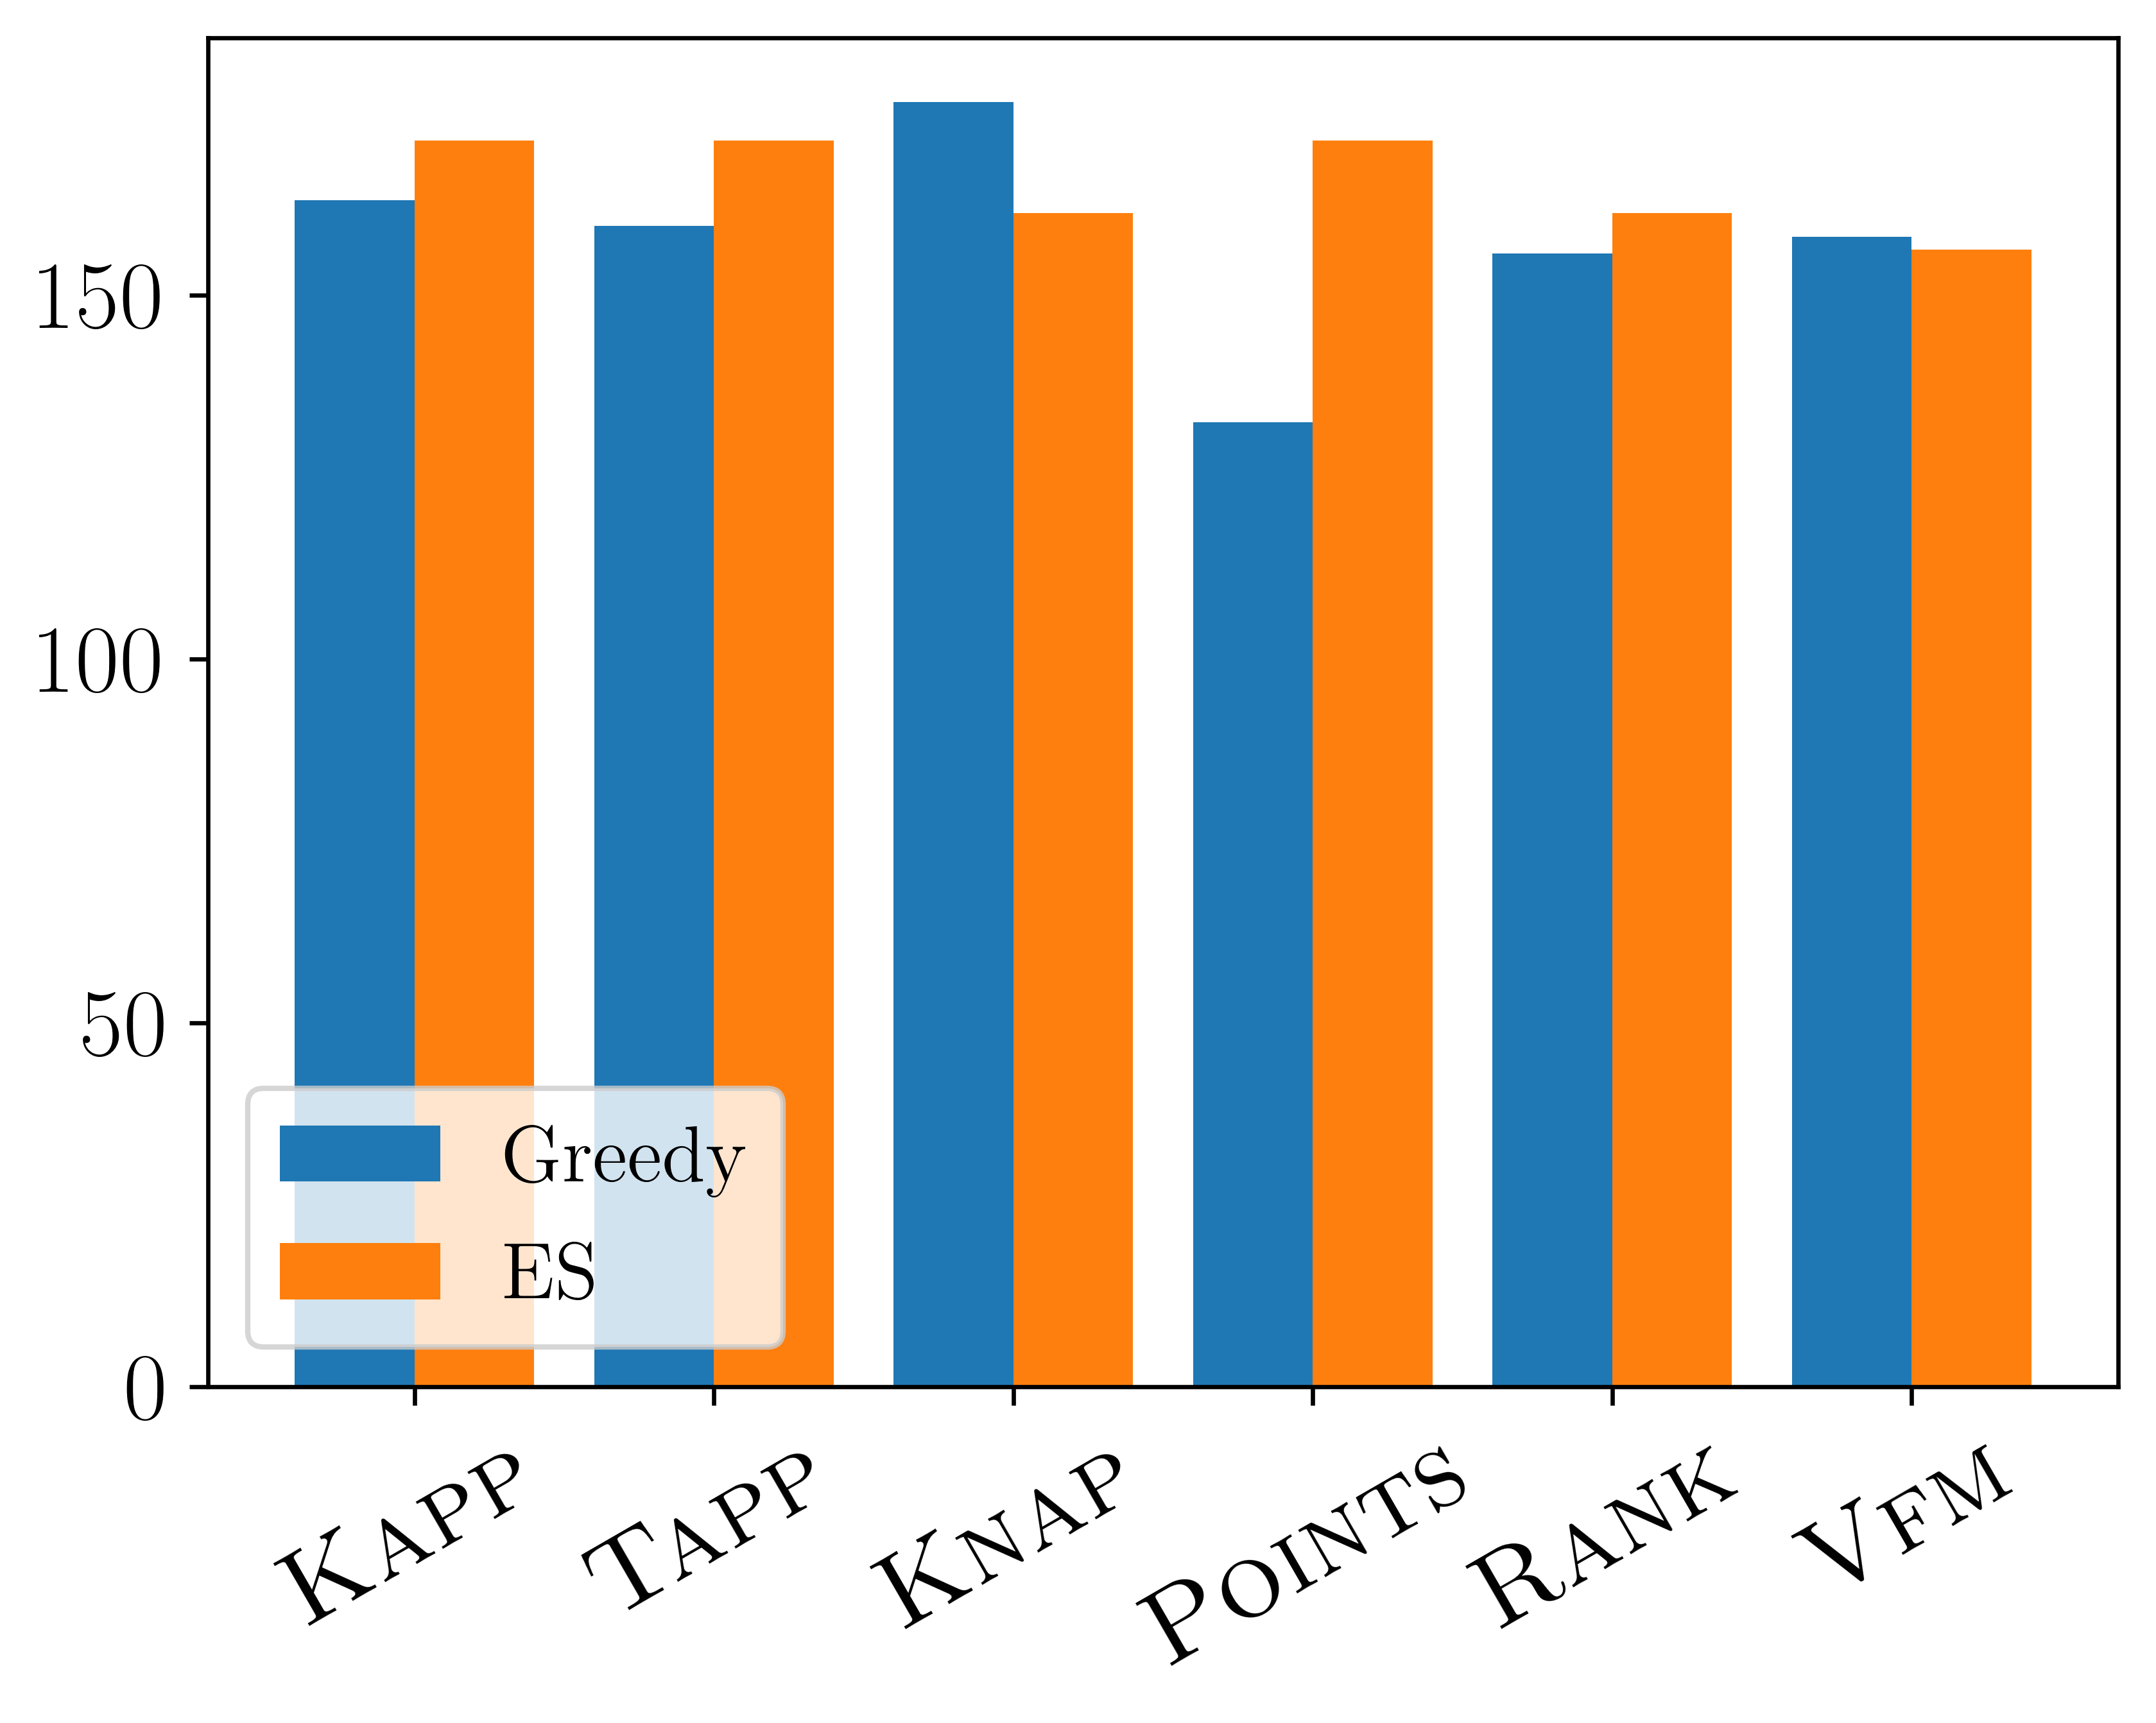
\includegraphics[width=7.5cm]{experiment/k_approval_welfare.png}
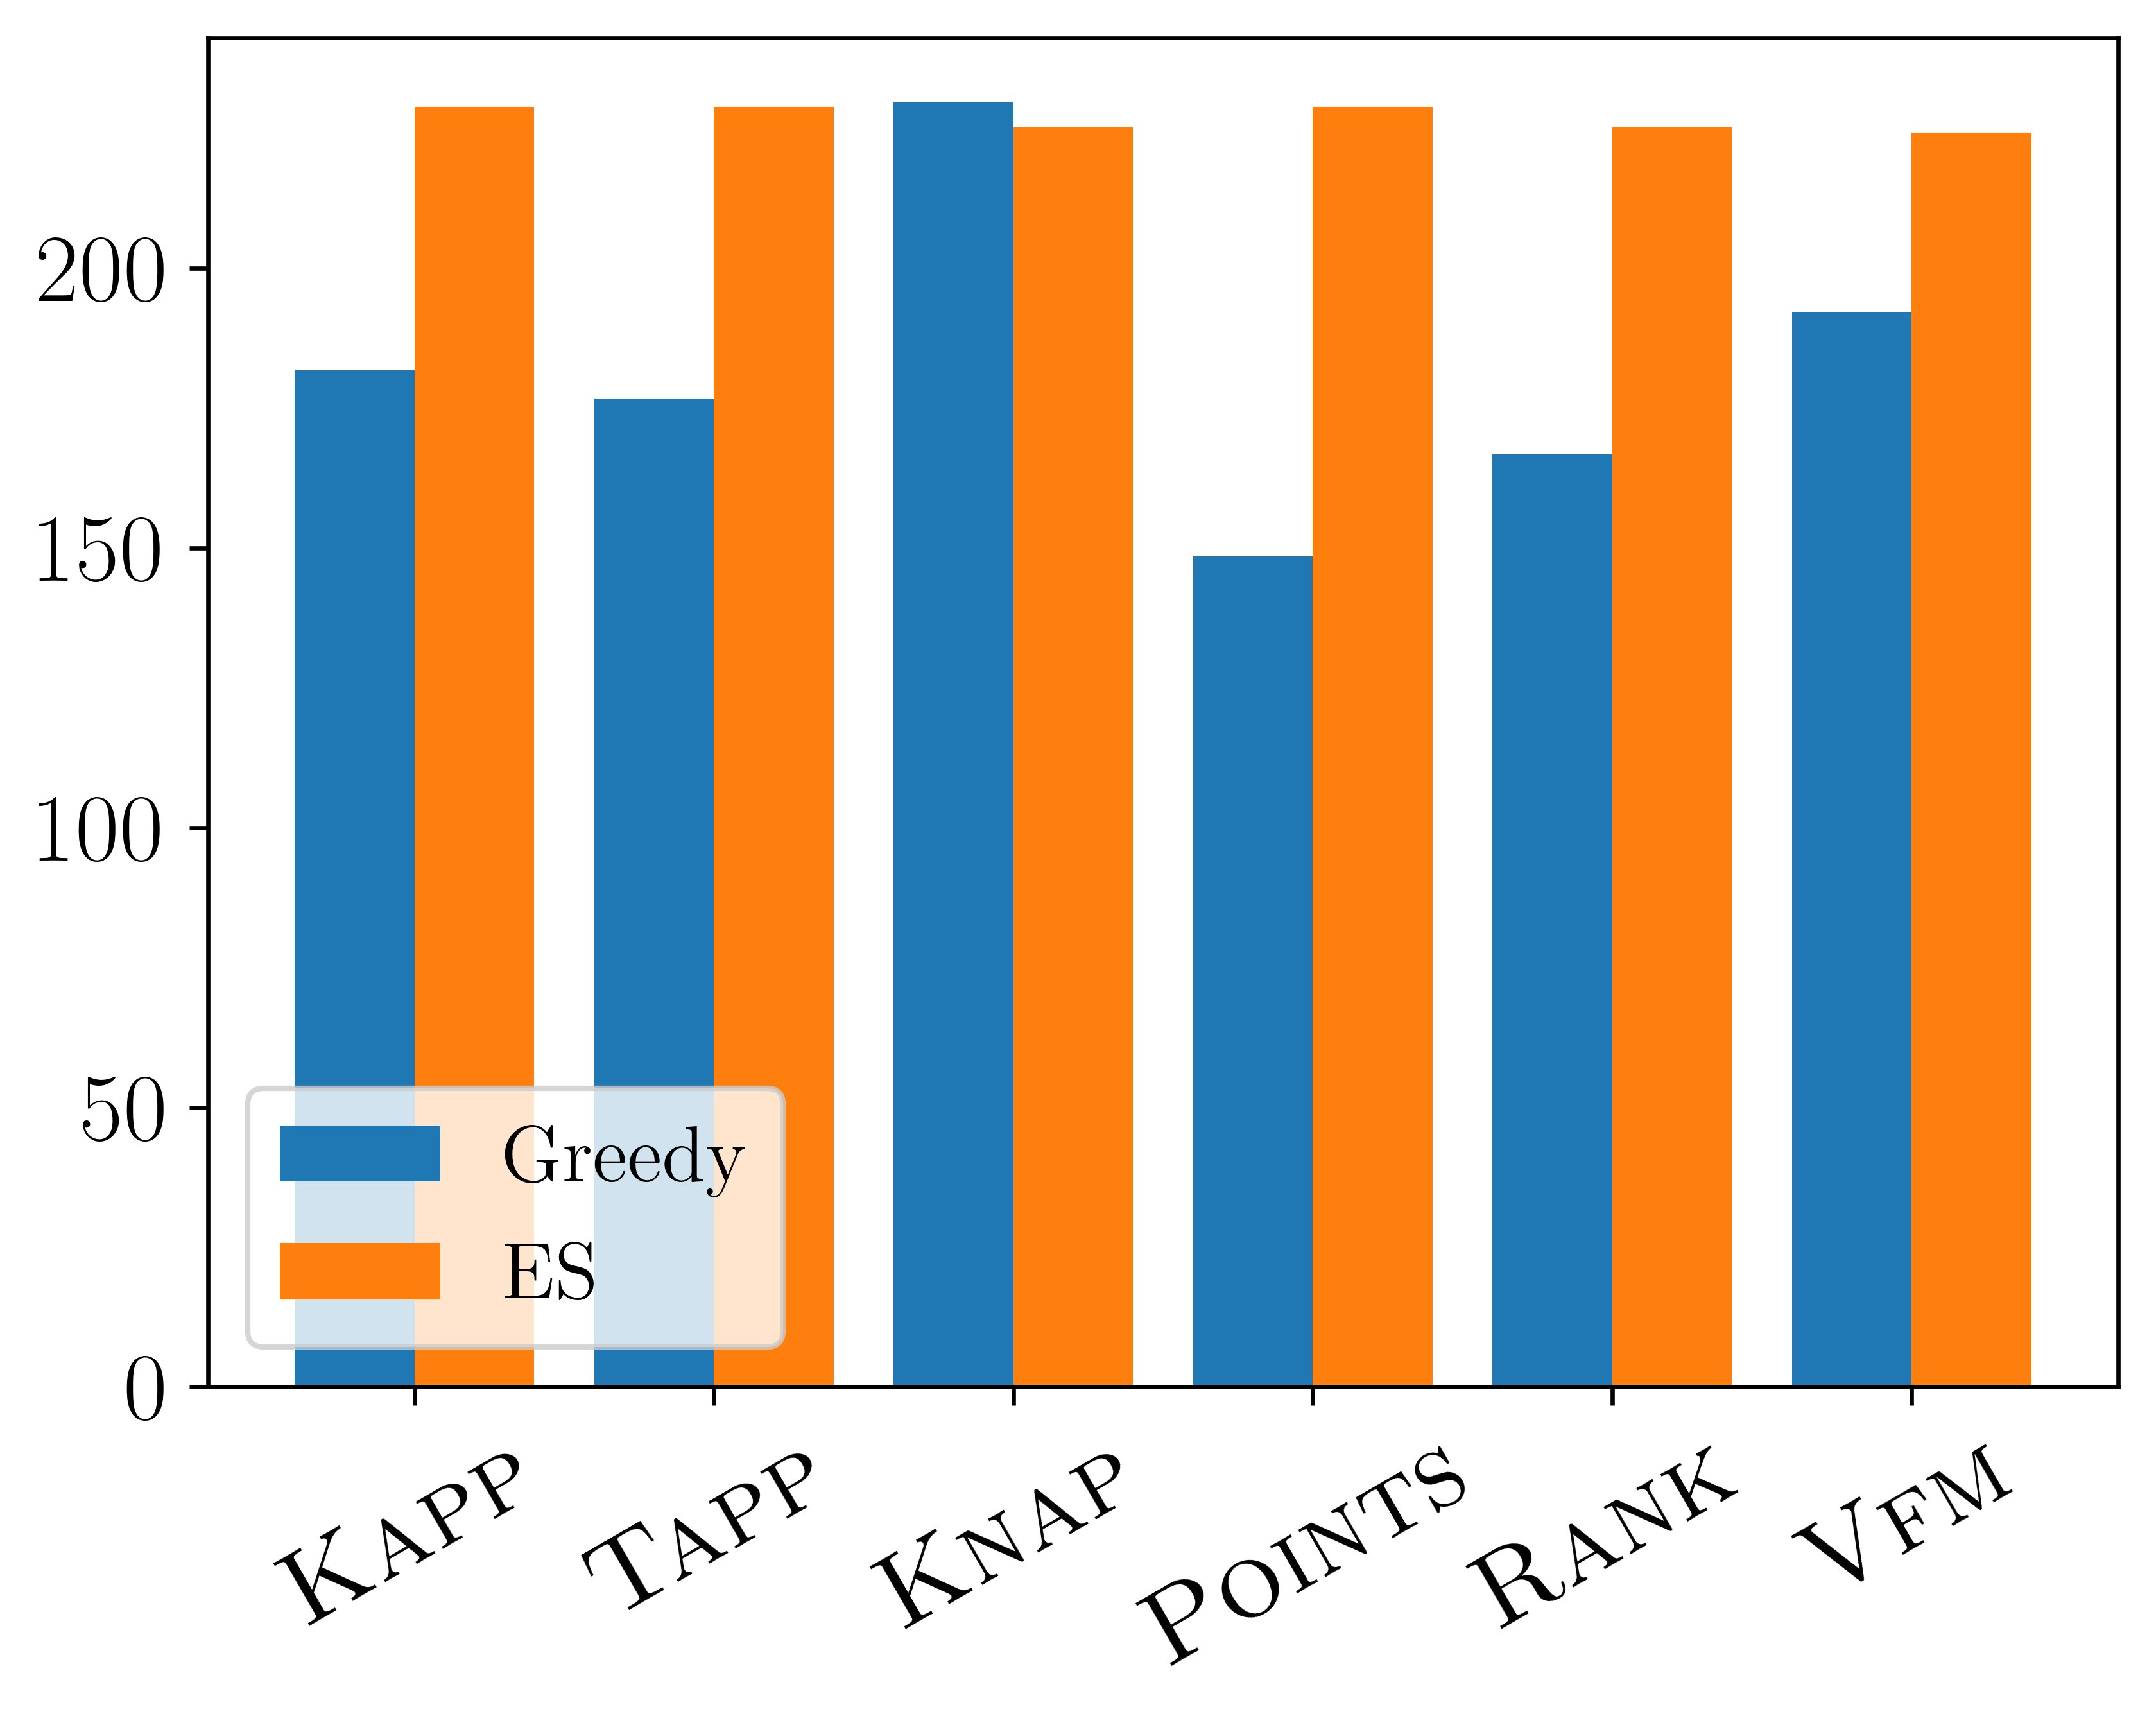
\includegraphics[width=7.5cm]{experiment/Knapsack_welfare.png}
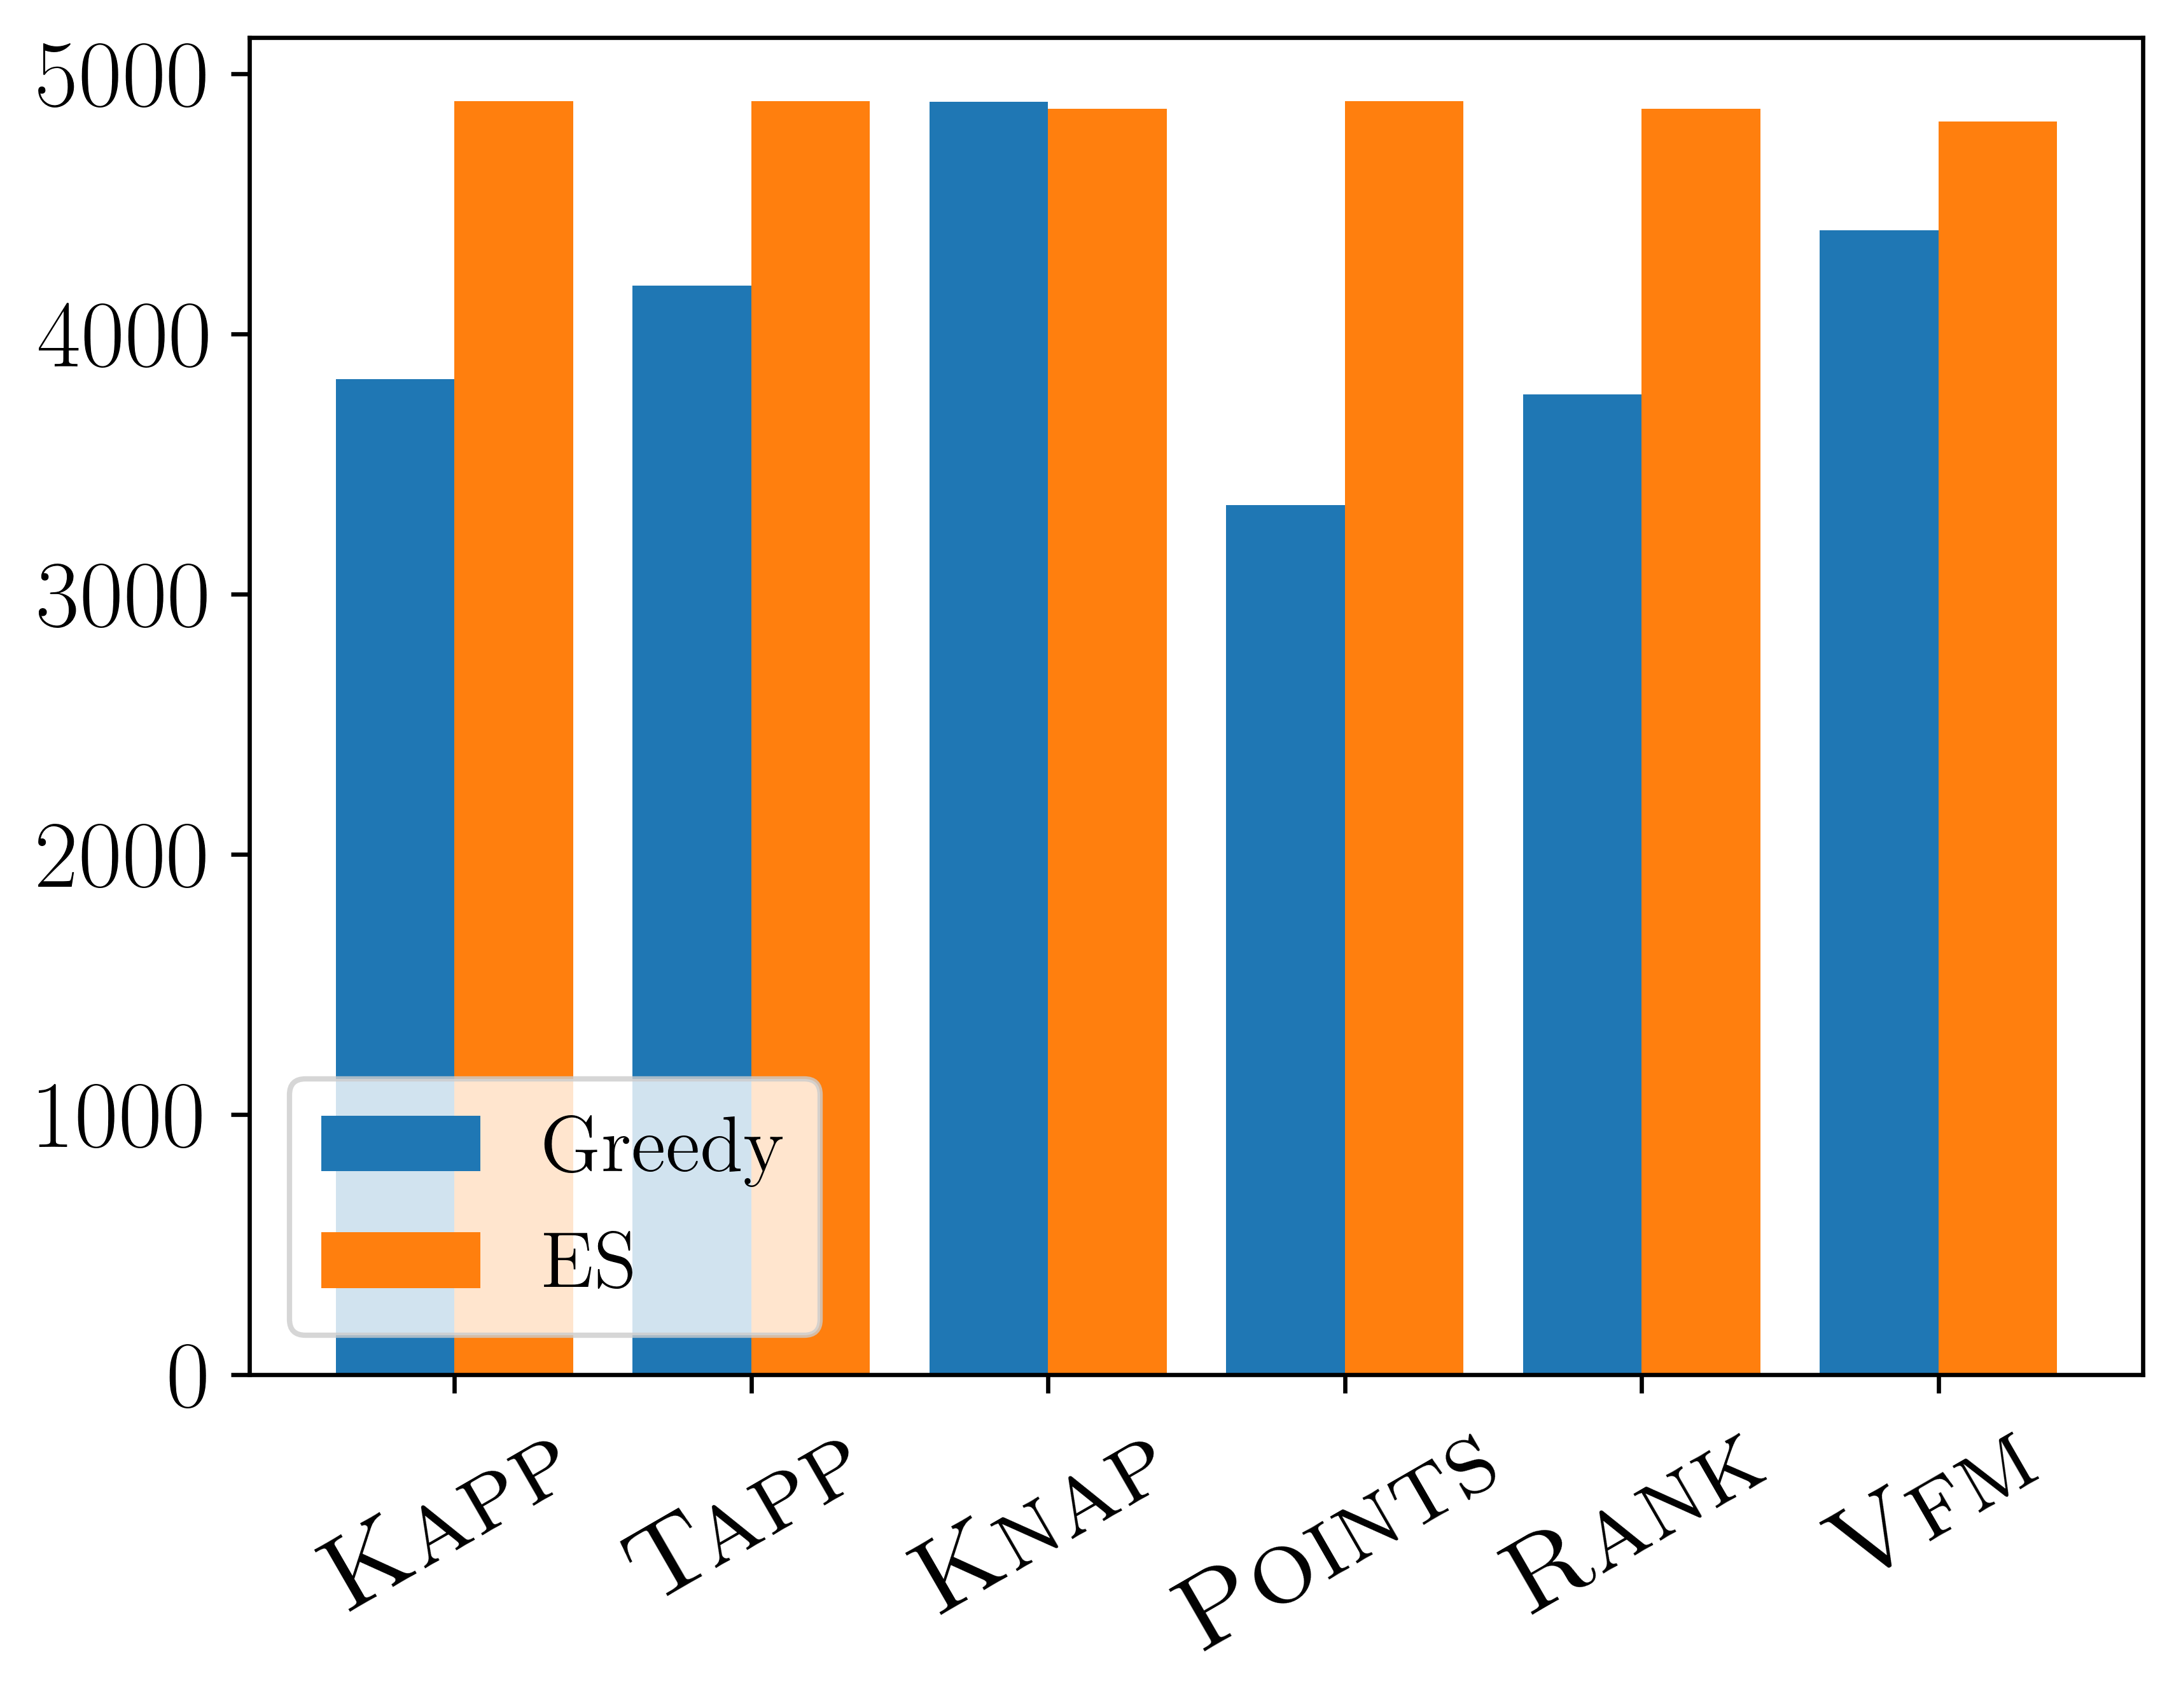
\includegraphics[width=7.5cm]{experiment/Ranking_value_welfare.png}
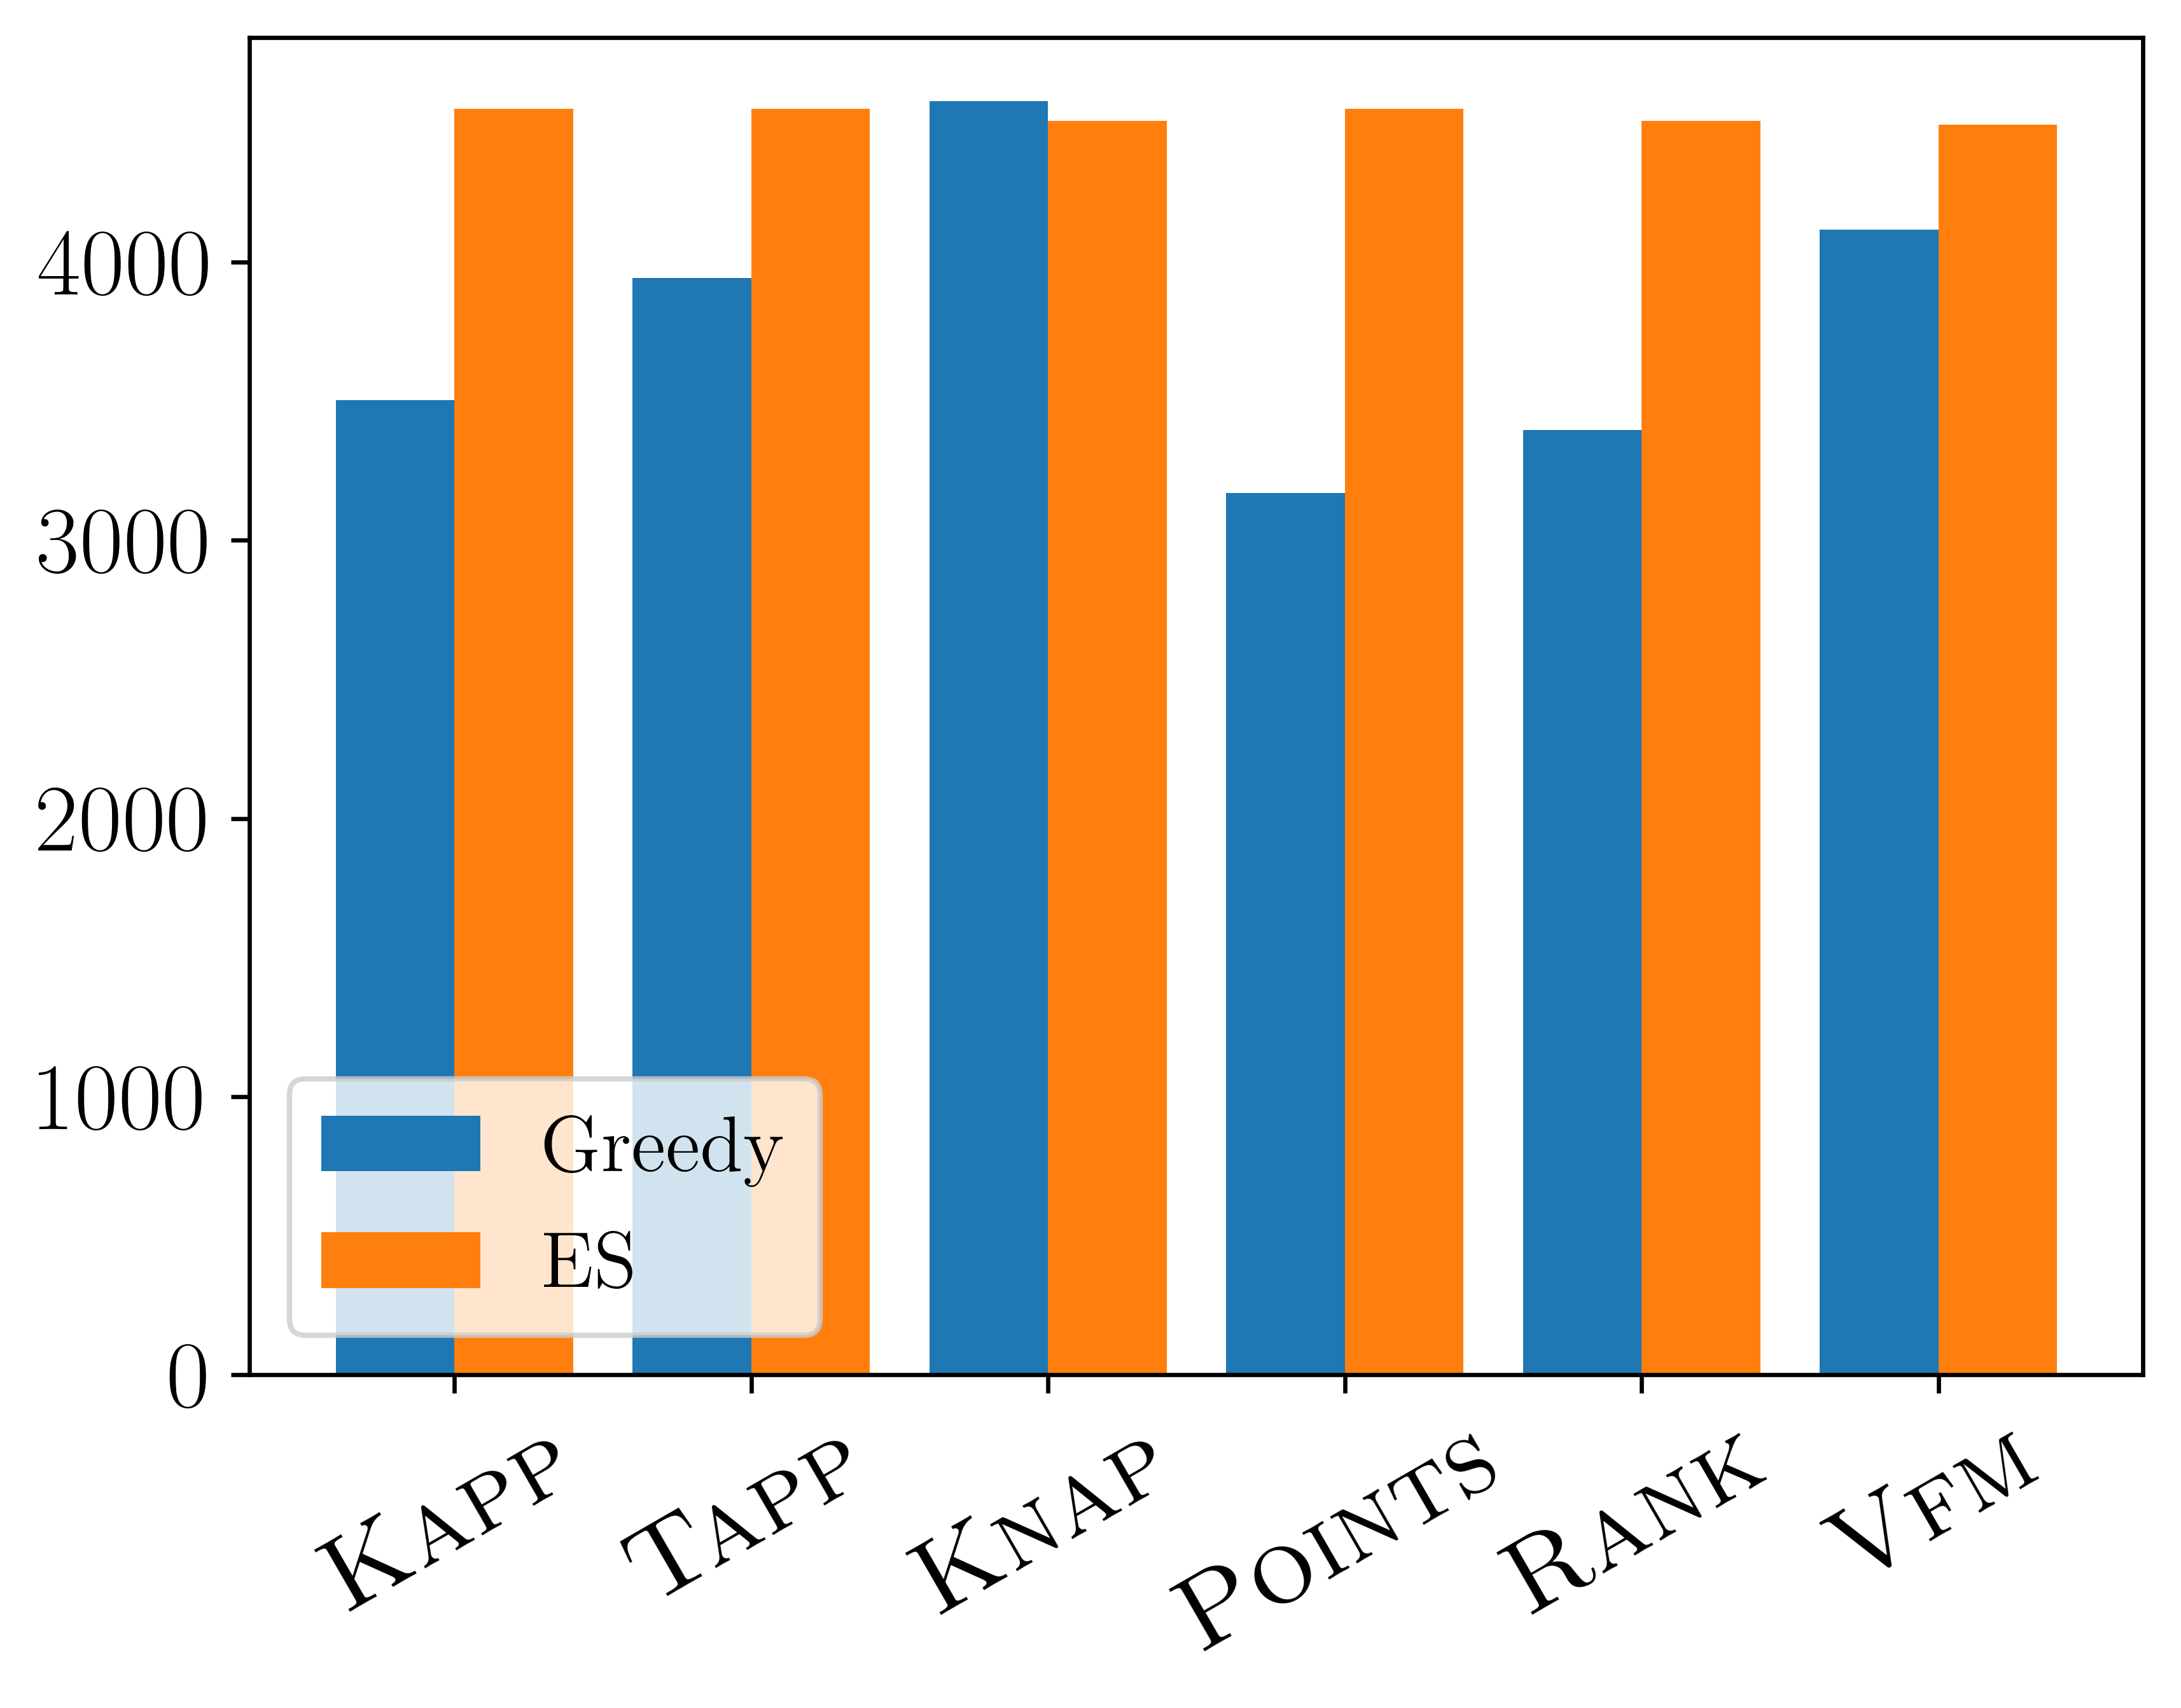
\includegraphics[width=7.5cm]{experiment/Ranking_value_money_welfare.png}
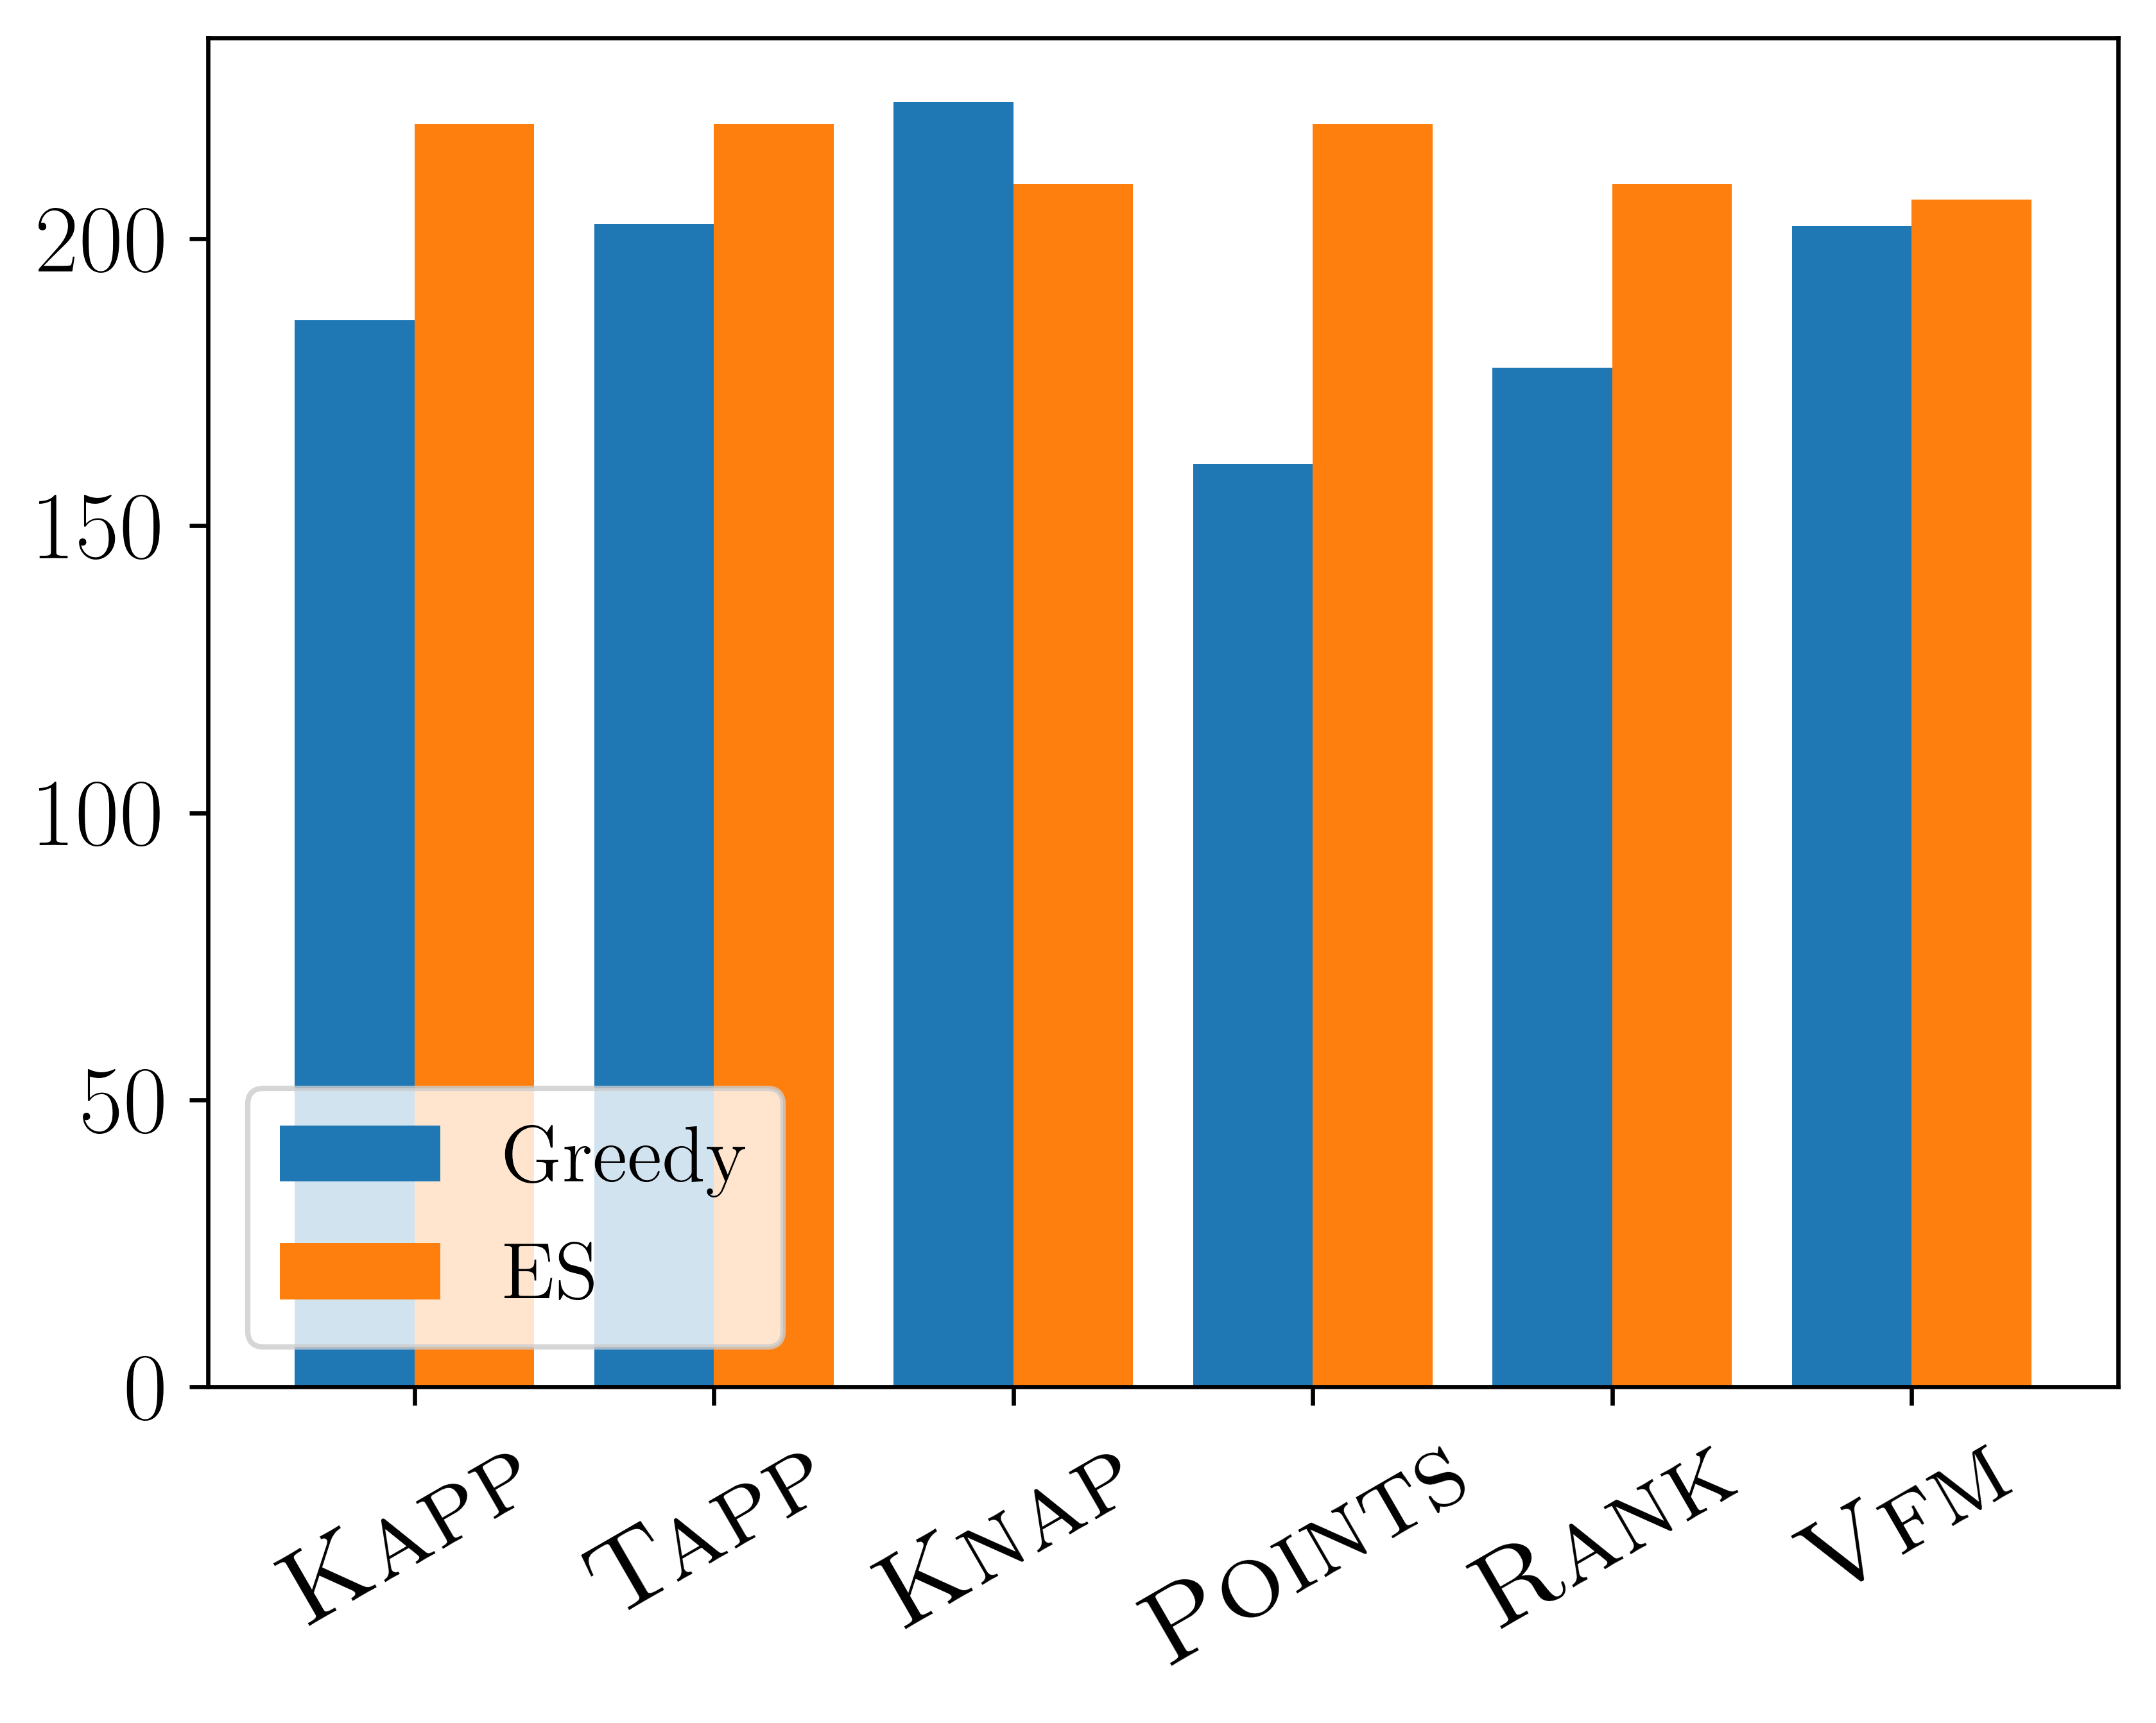
\includegraphics[width=7.5cm]{experiment/Threshold_welfare.png}
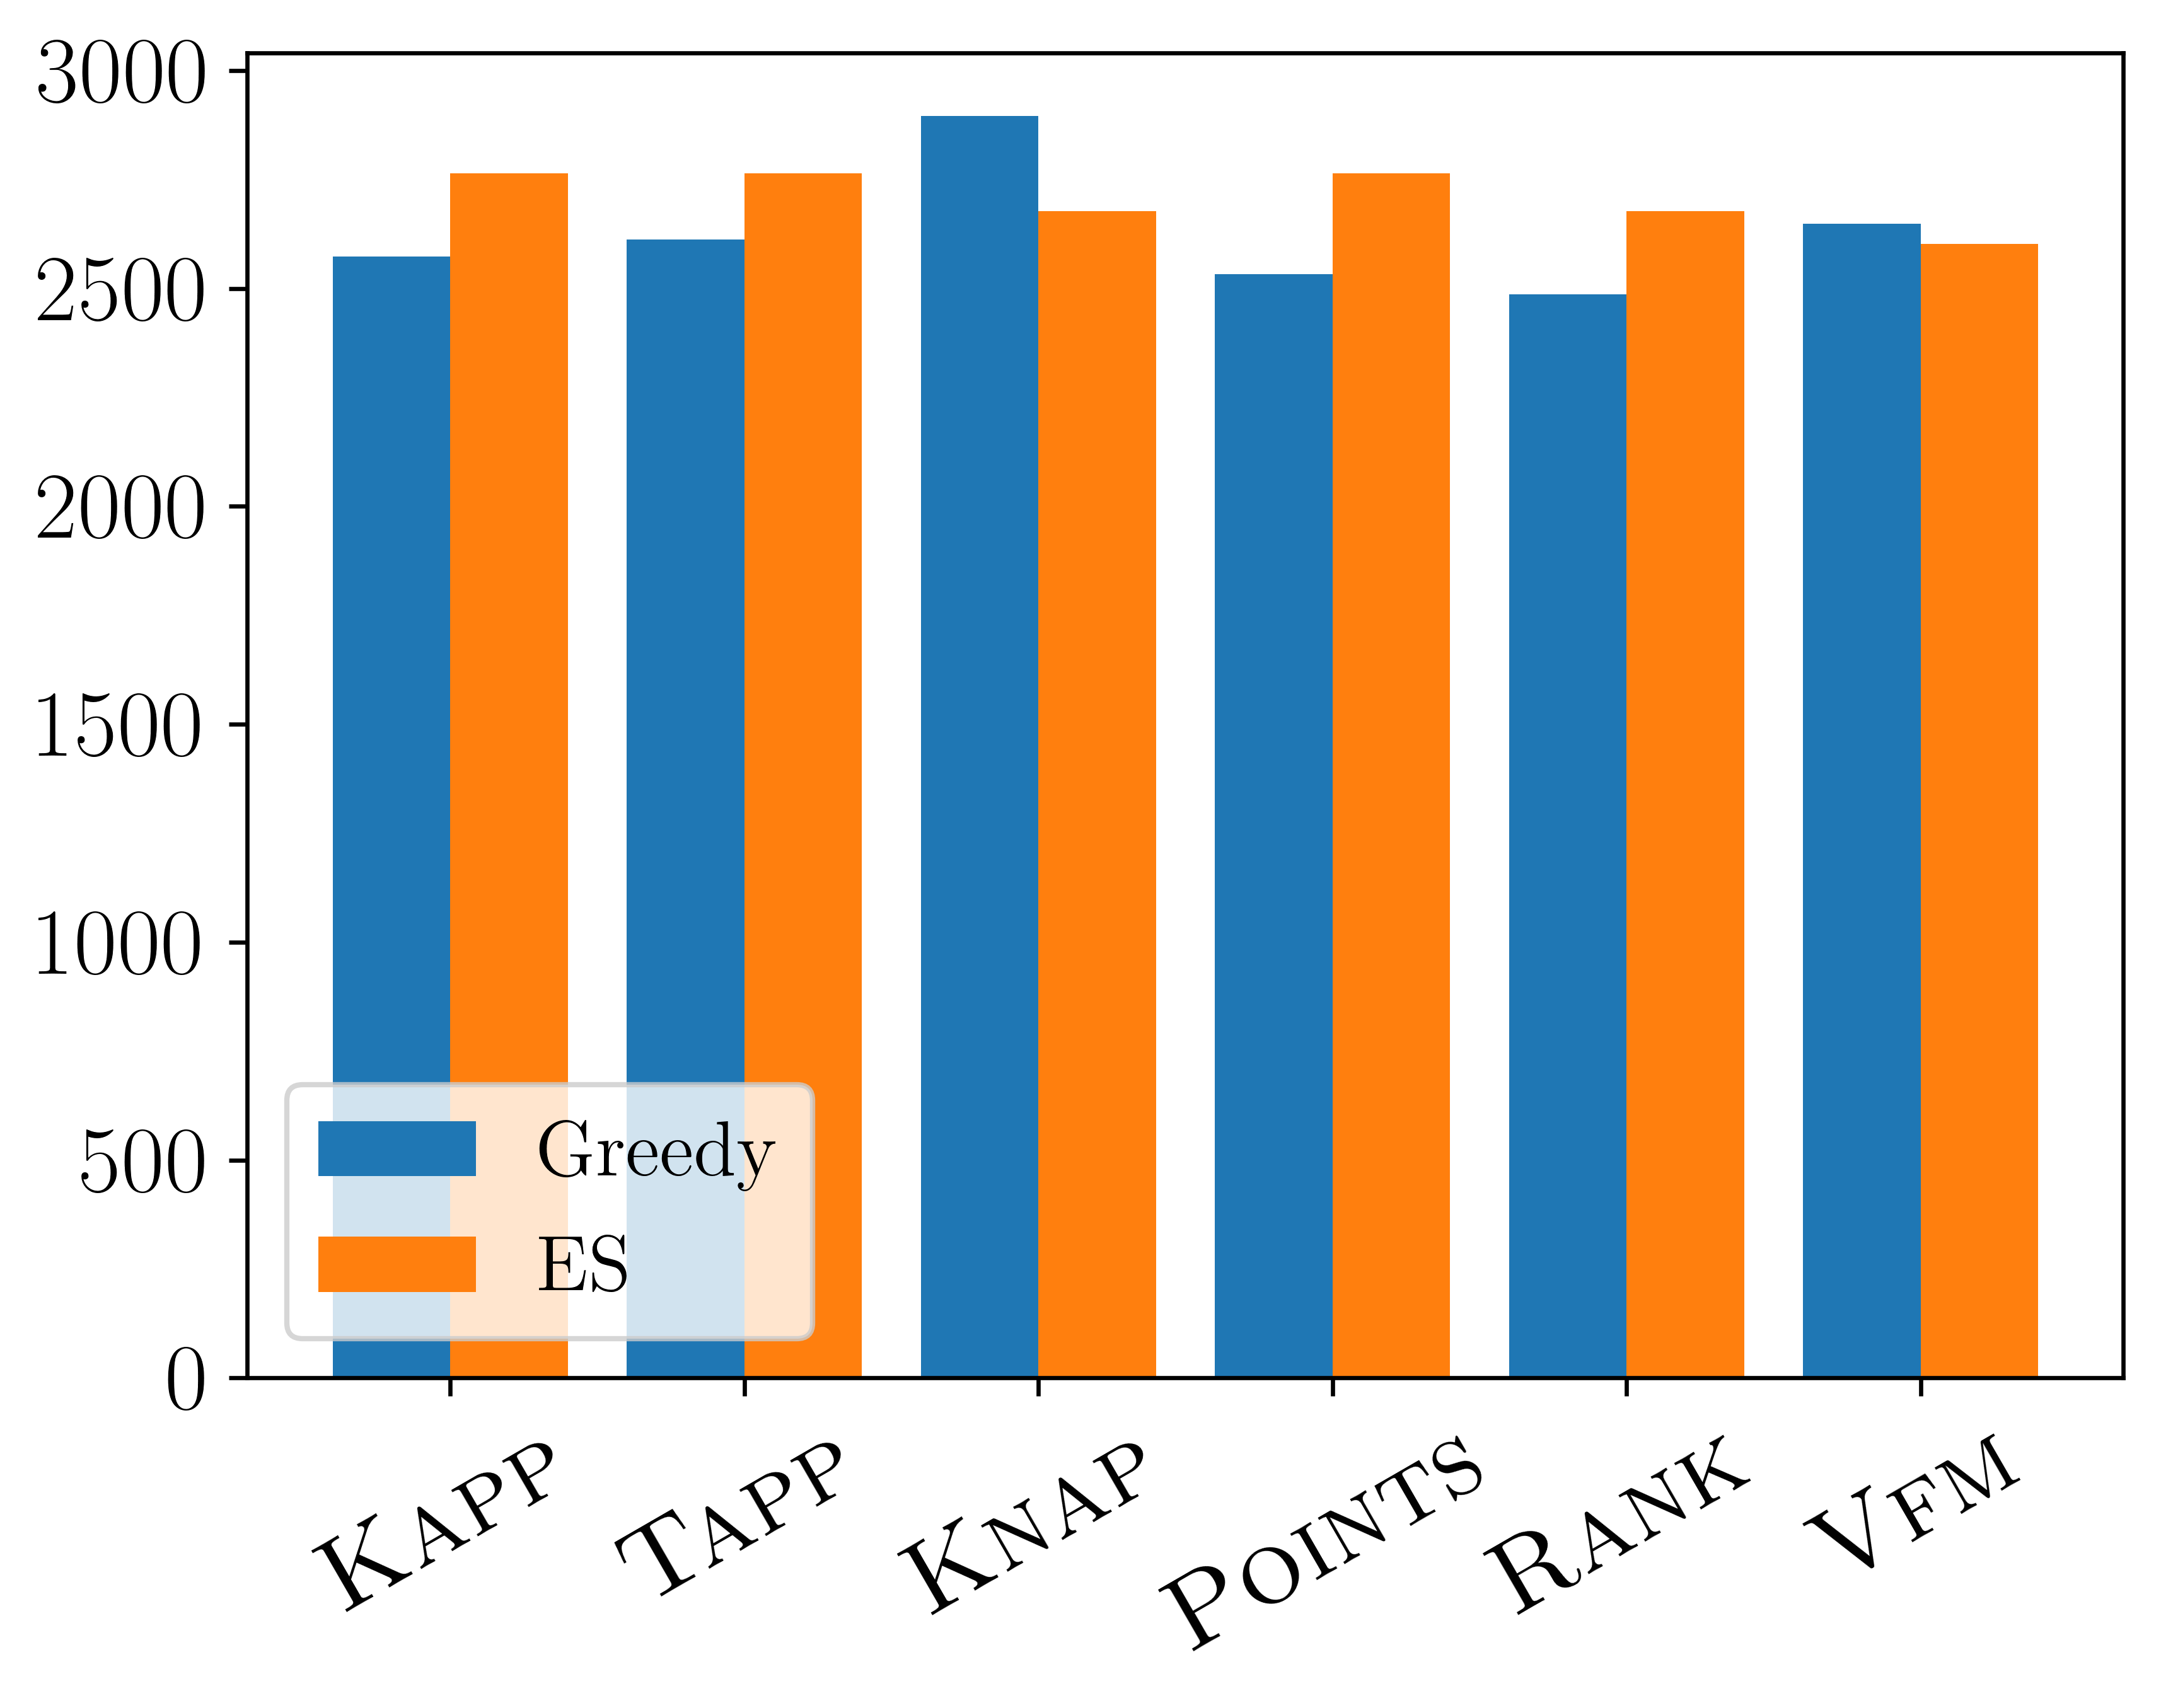
\includegraphics[width=7.5cm]{experiment/Utilities_welfare.png}
\caption{Average social welfare for each type of input format voters.
}\label{fig:all_welfare}
\end{center}
\end{figure}

\begin{figure}[!htbp]
\begin{center}
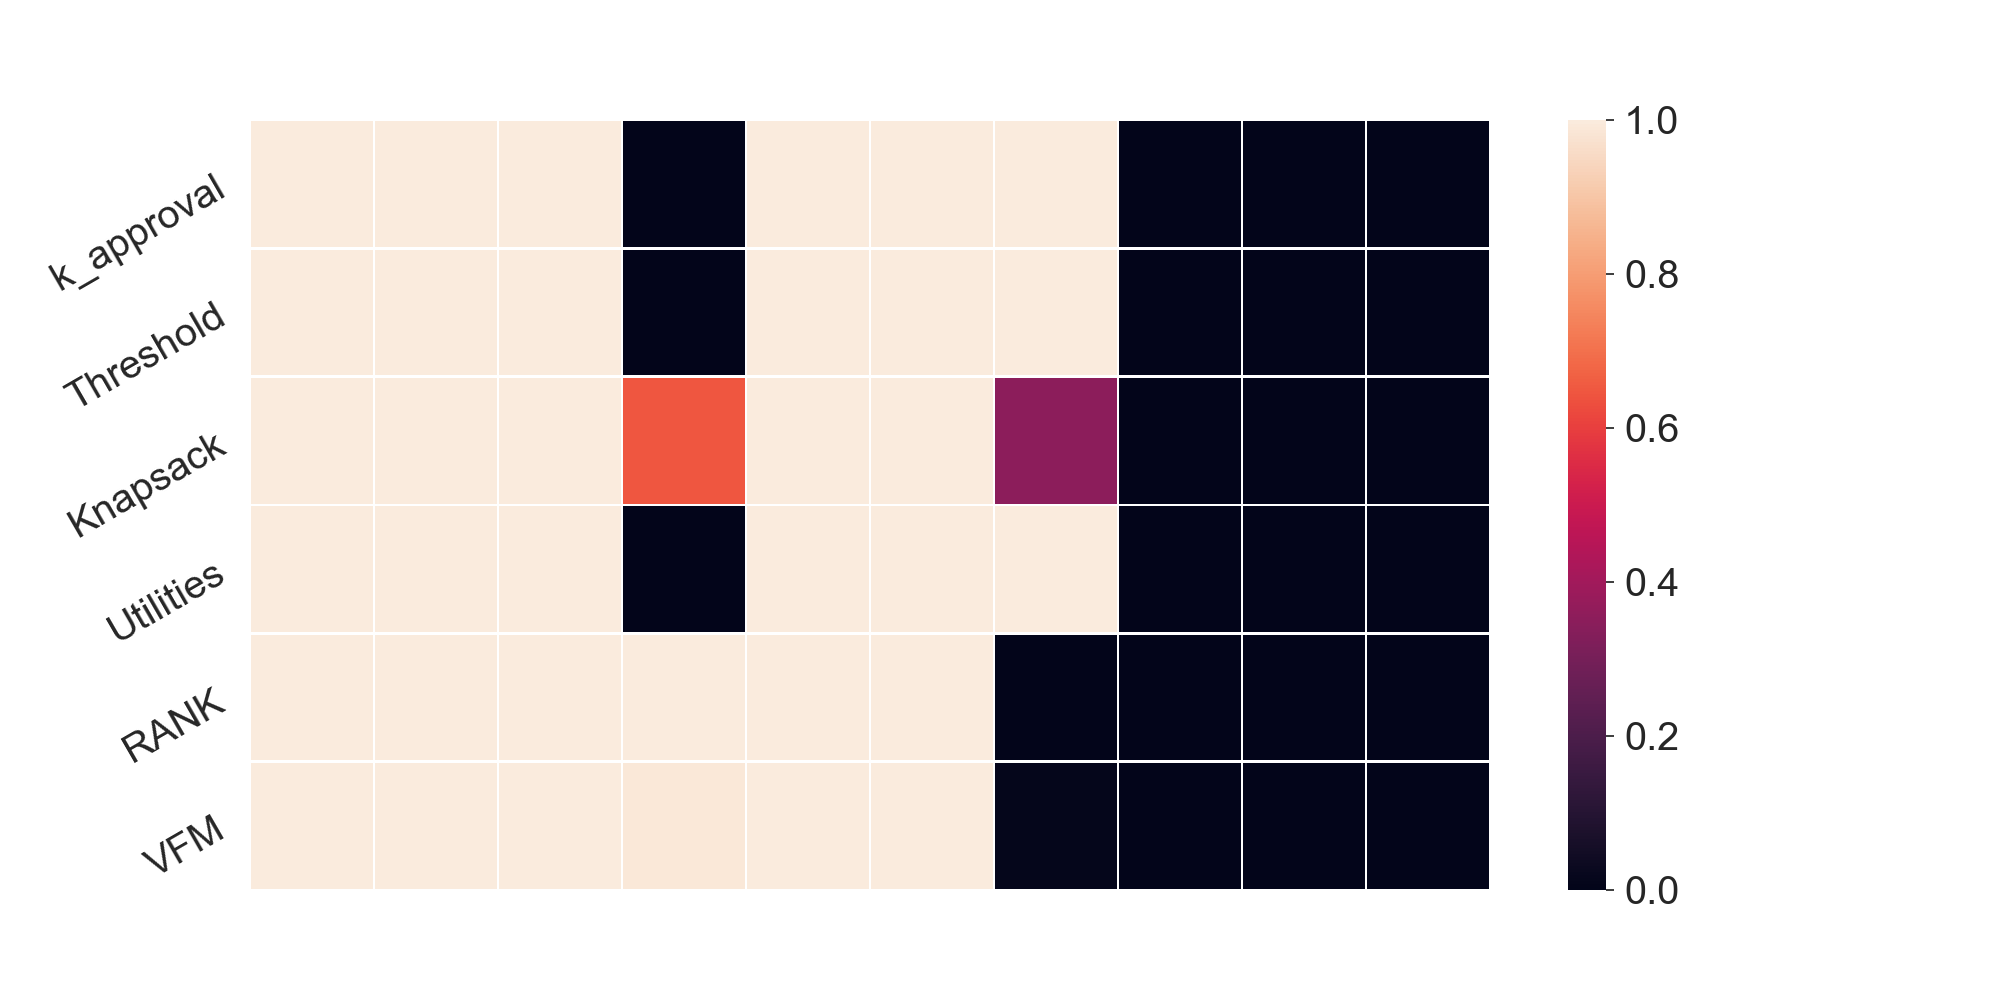
\includegraphics[width=18cm]{experiment/election_3_rx.png}
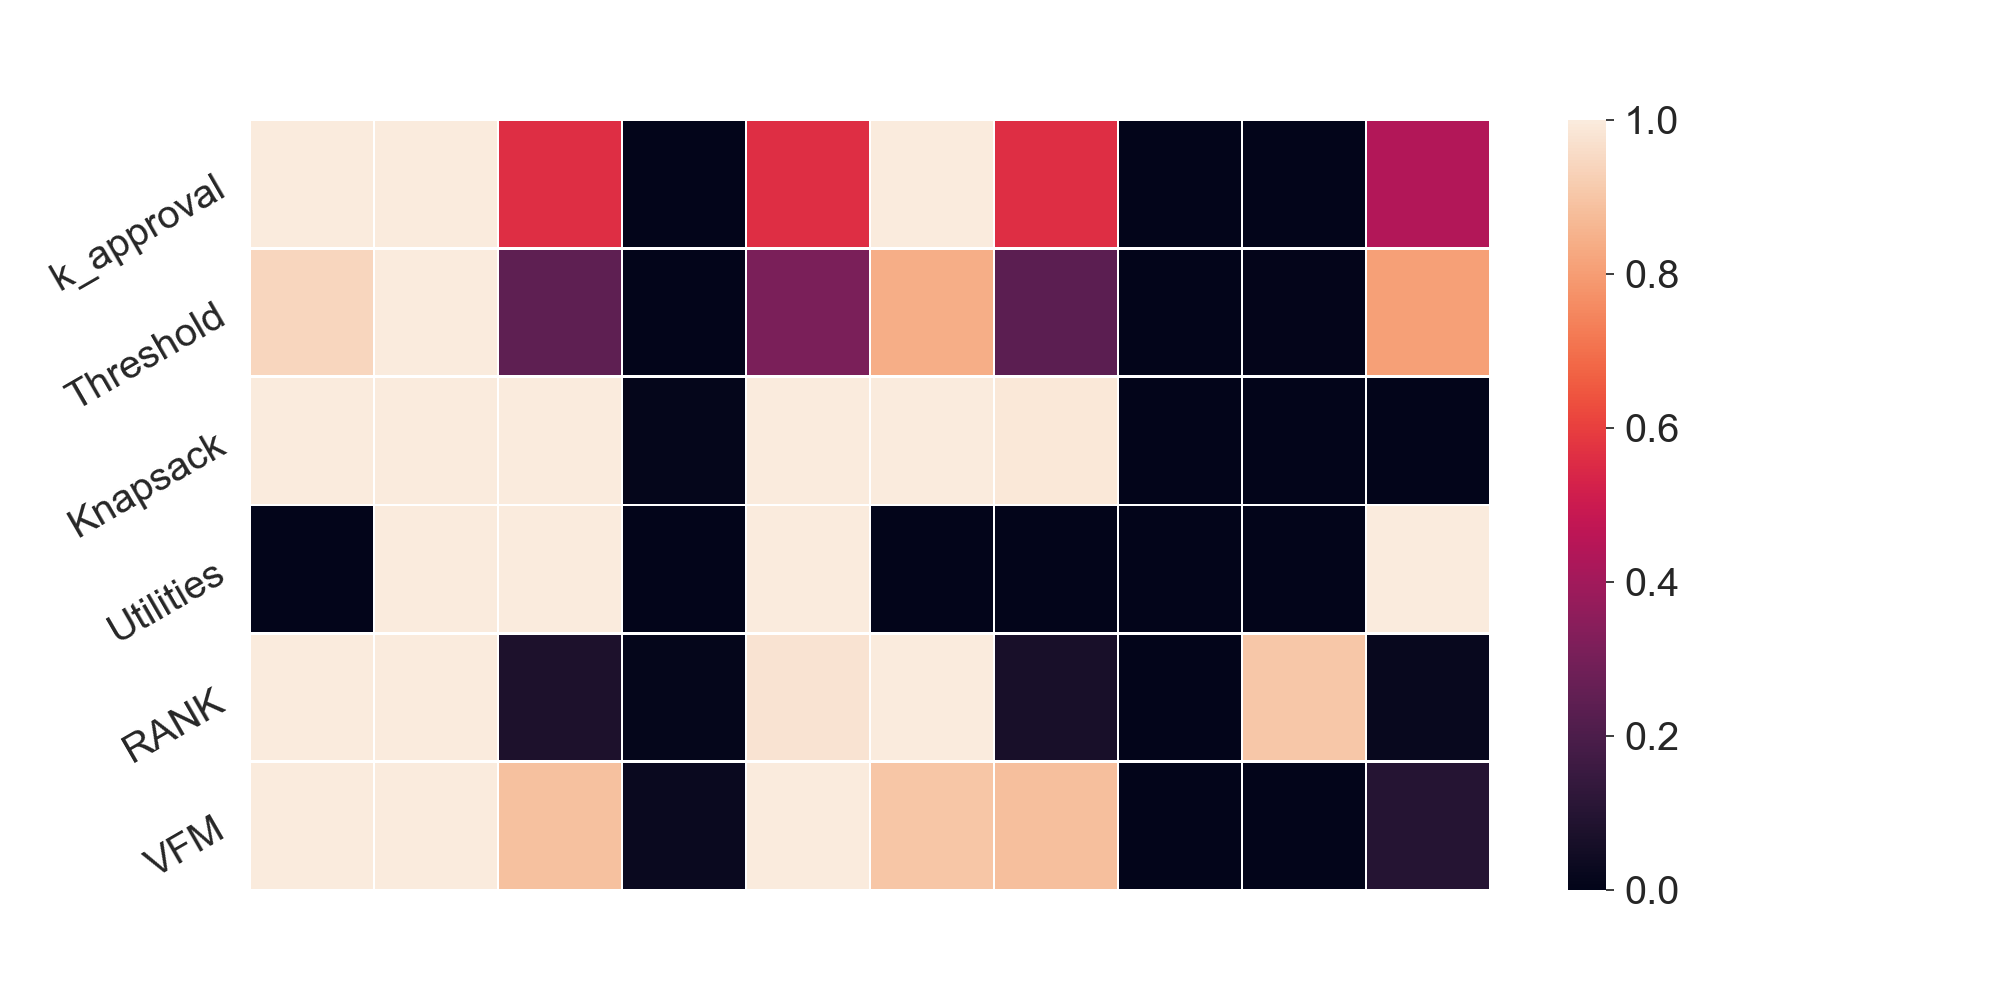
\includegraphics[width=18cm]{experiment/election_3_greedy.png}
\caption{Percentage of instances where each projects was selected for RX (top) and greedy (bottom)
aggregation for election 3.
}\label{fig:stability3}
\end{center}
\end{figure}

\begin{figure}[!htbp]
\begin{center}
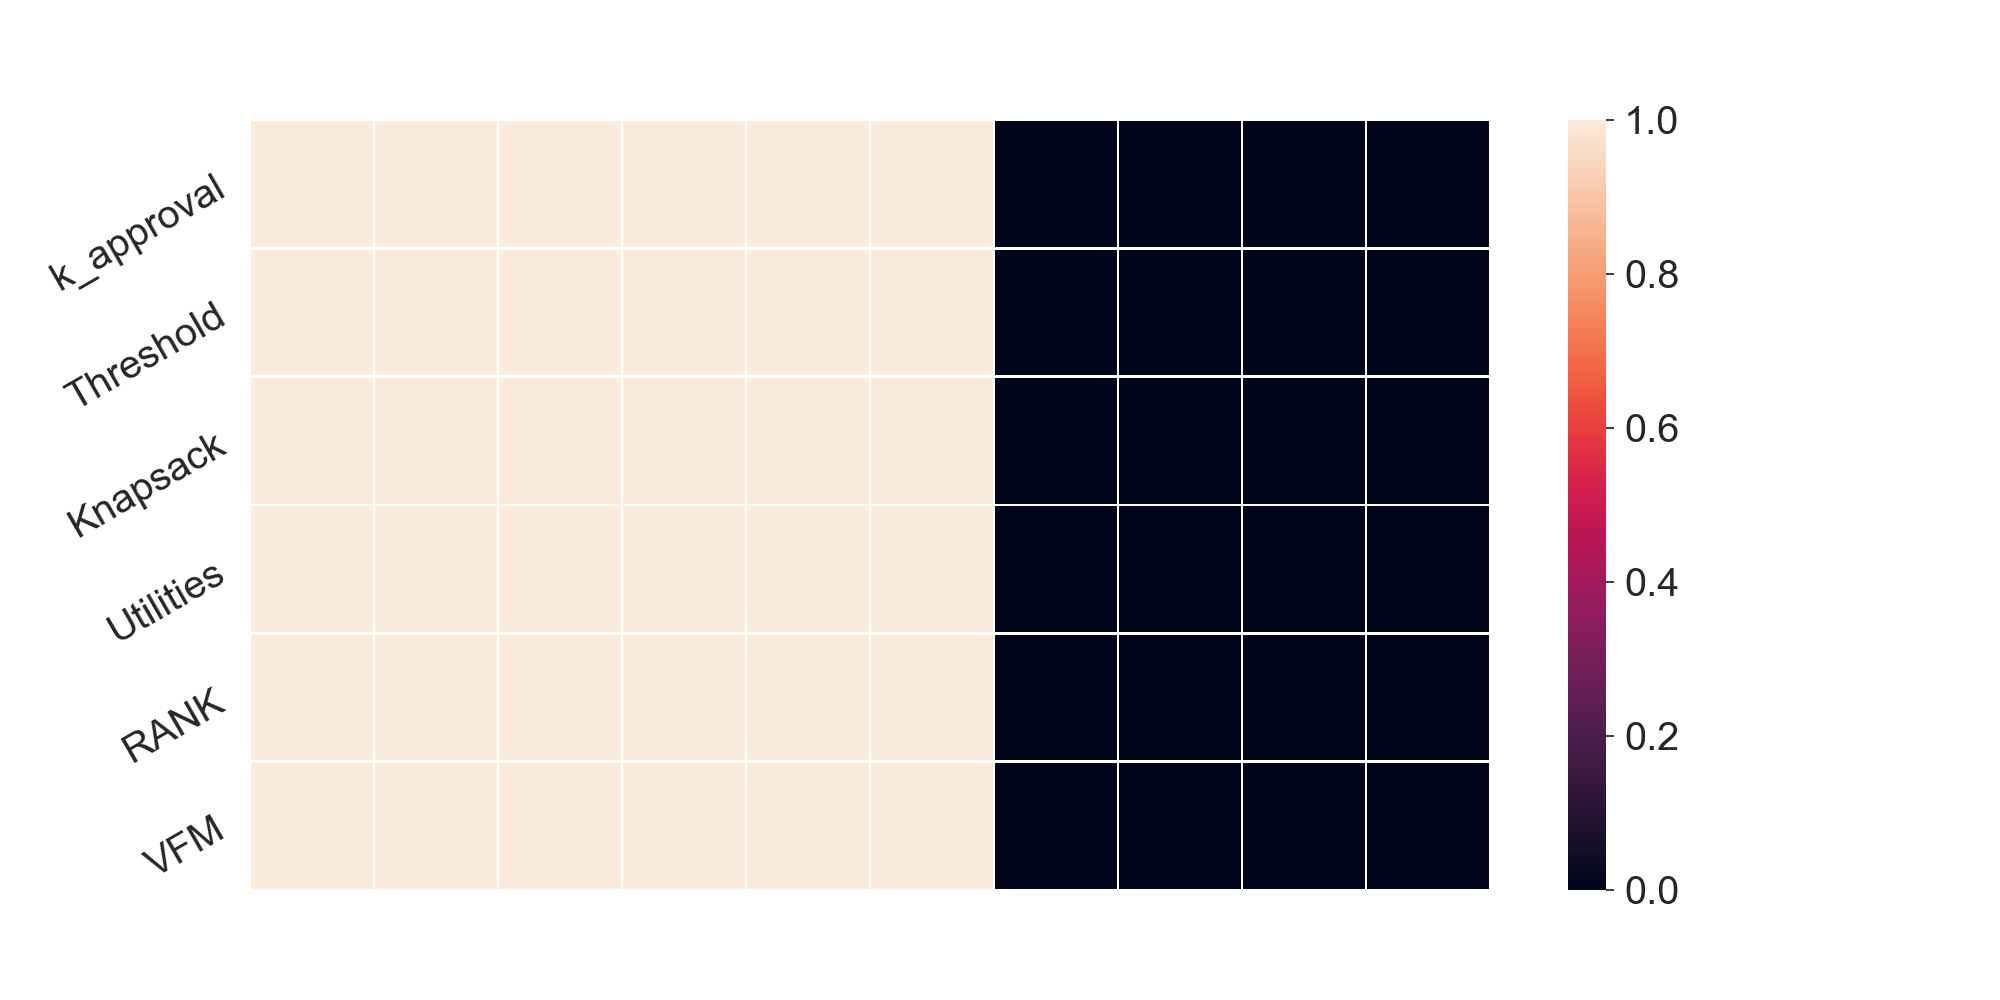
\includegraphics[width=18cm]{experiment/election_6_rx.png}
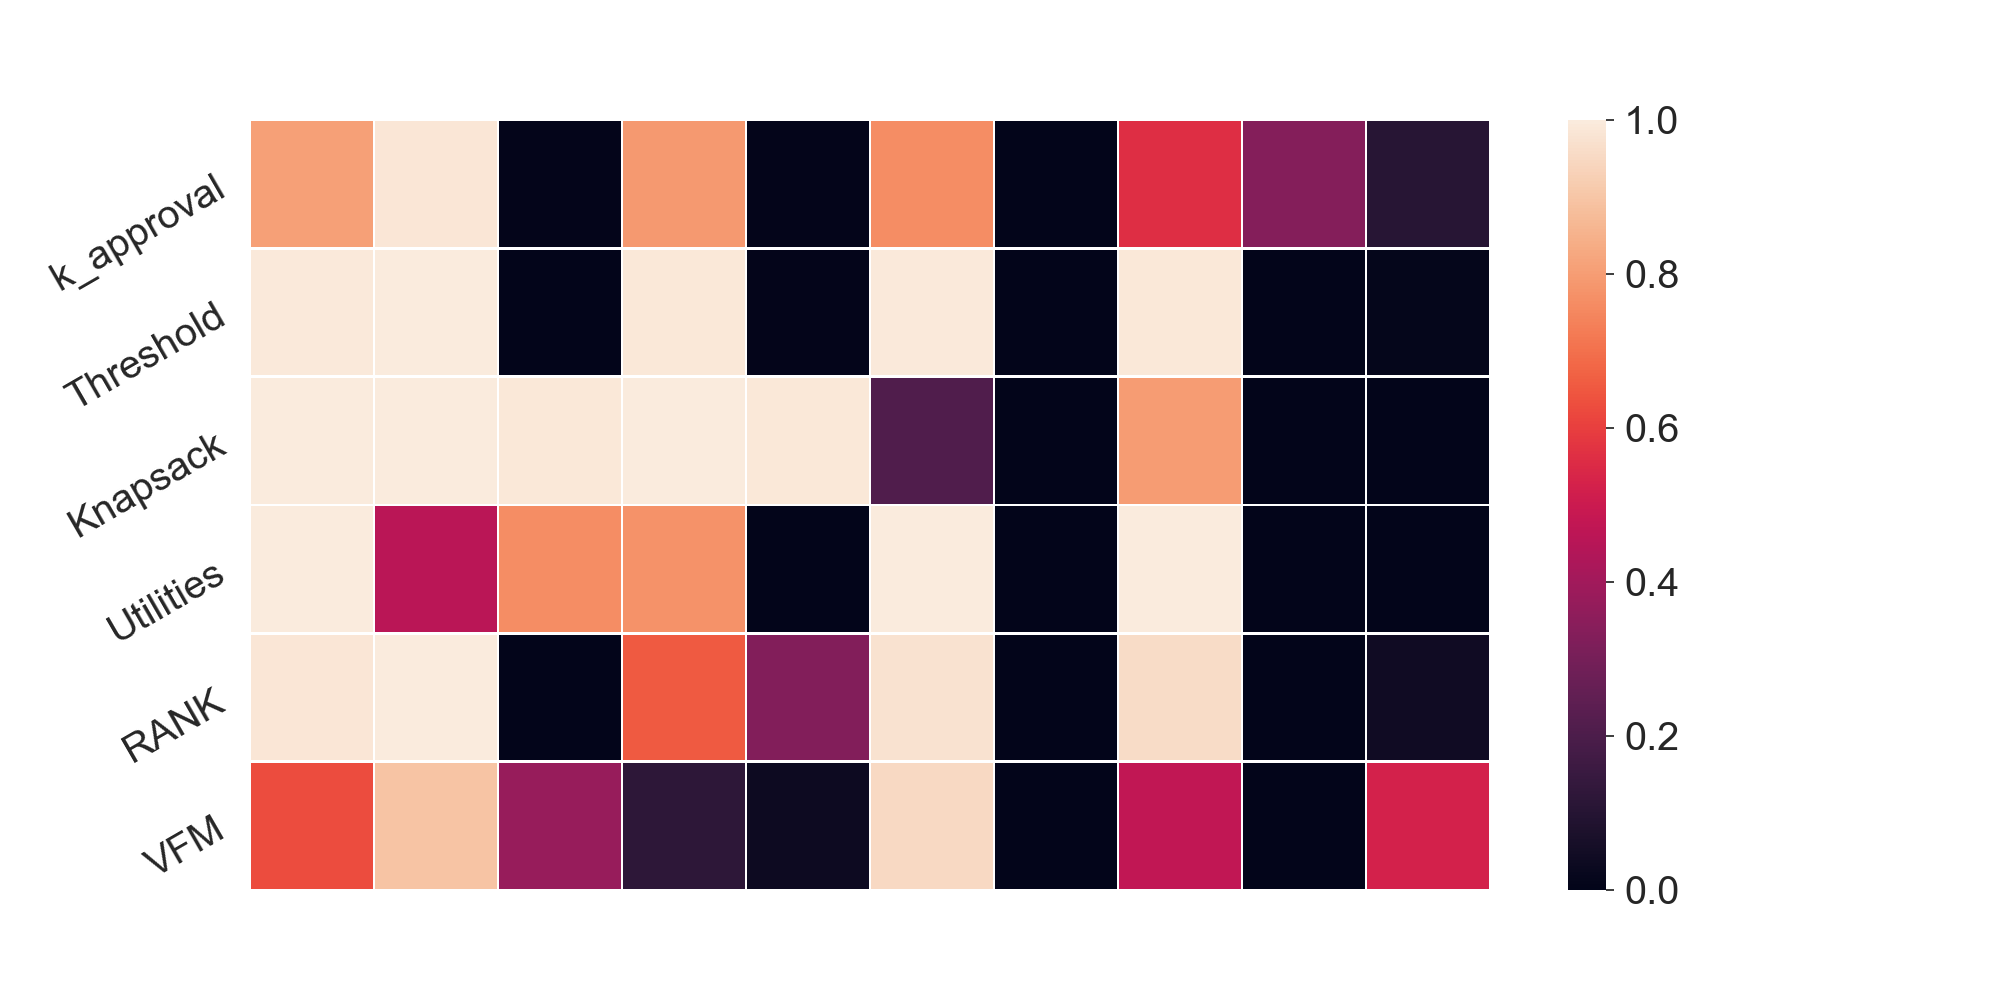
\includegraphics[width=18cm]{experiment/election_6_greedy.png}
\caption{Percentage of instances where each projects was selected for RX (top) and greedy (bottom)
aggregation for election 6.
}\label{fig:stability6}
\end{center}
\end{figure}

\begin{figure}[!htbp]
\begin{center}

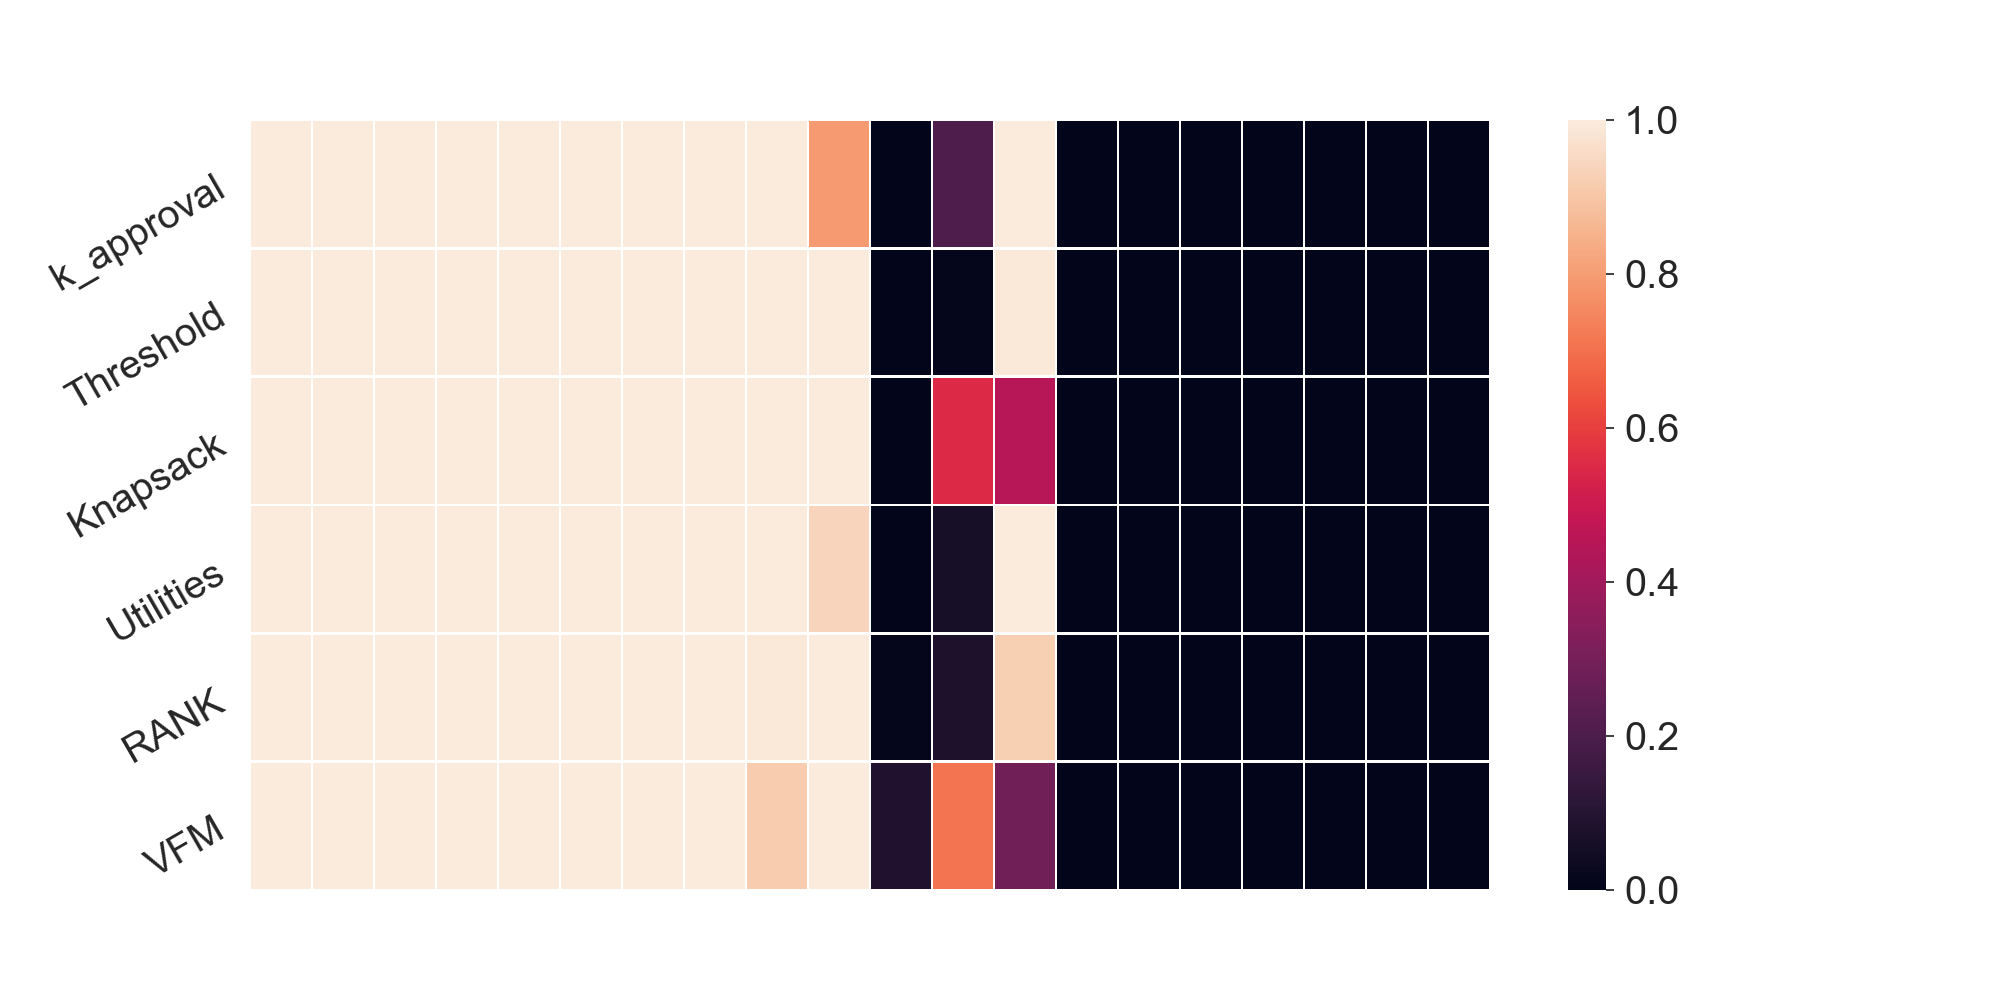
\includegraphics[width=18cm]{experiment/election_7_rx.png}
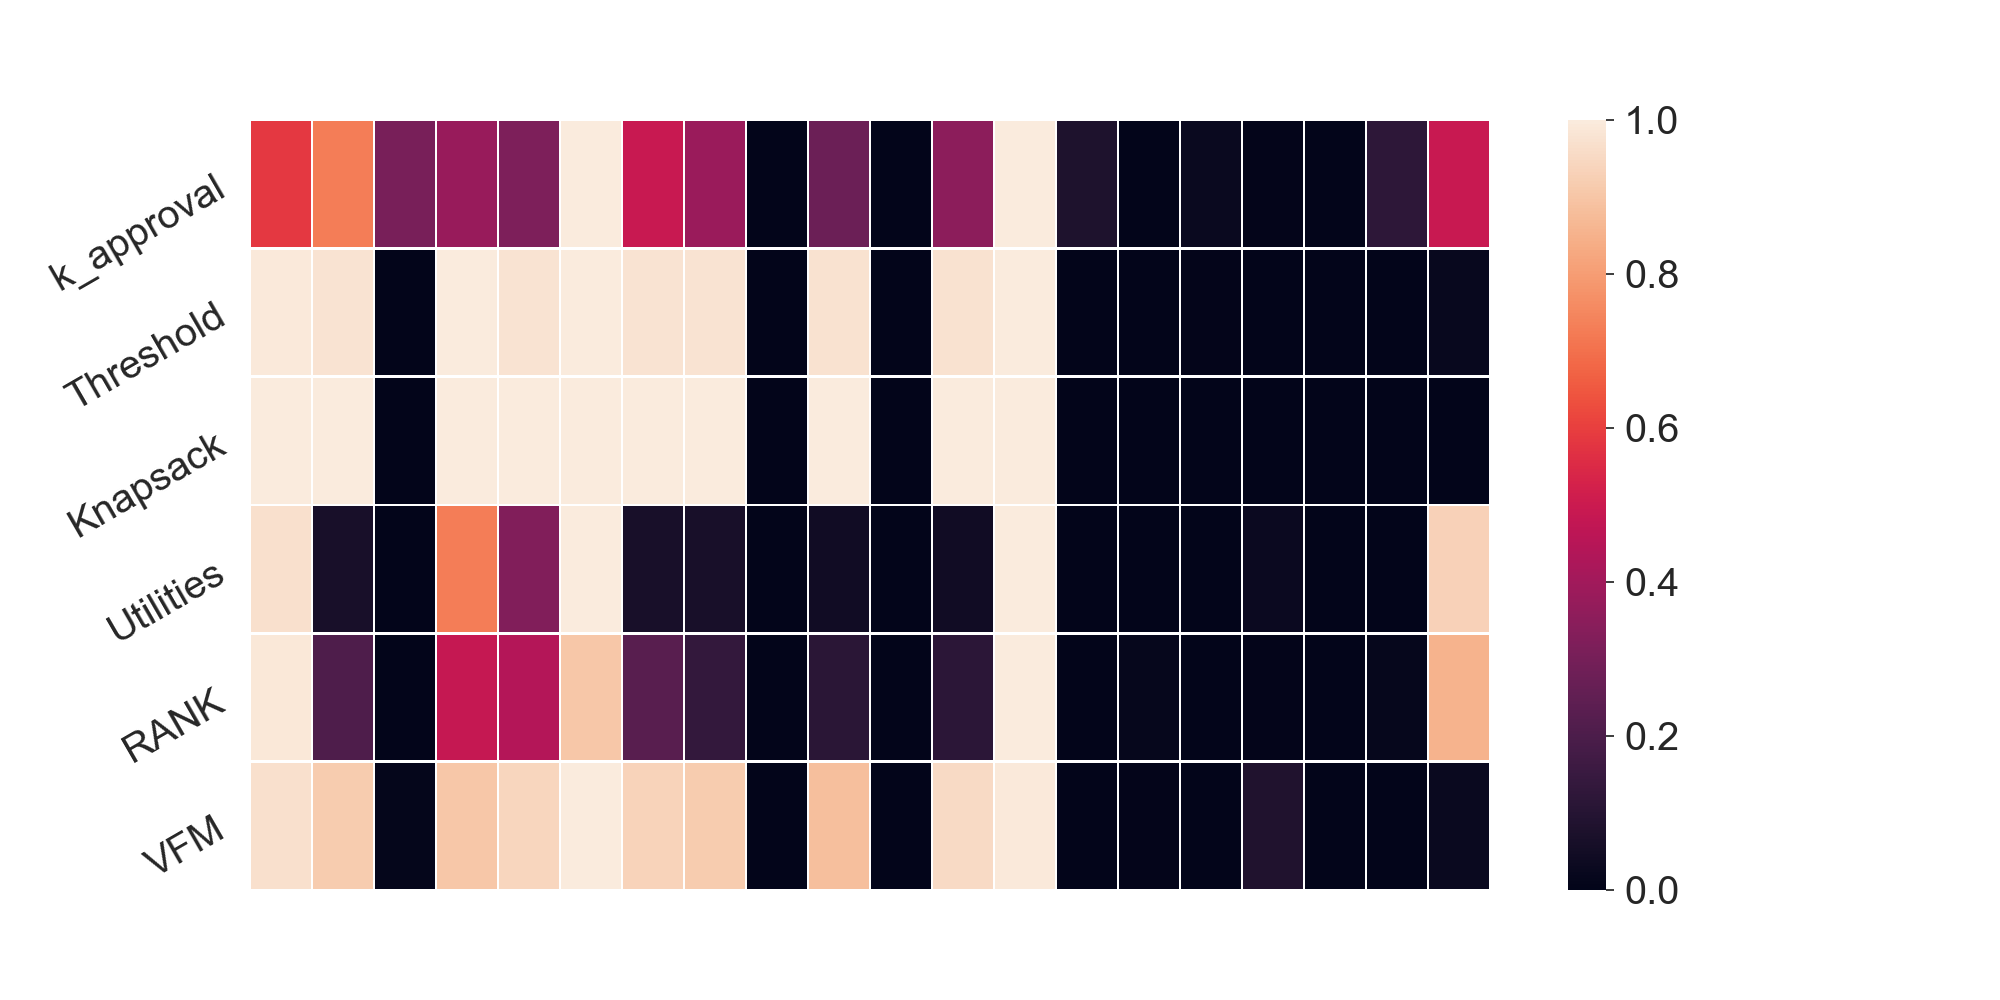
\includegraphics[width=18cm]{experiment/election_7_greedy.png}

\caption{Percentage of instances where each projects was selected for RX (top) and greedy (bottom)
aggregation for election 7.
}\label{fig:stability7}
\end{center}
\end{figure}

\begin{figure}[!htbp]
\begin{center}
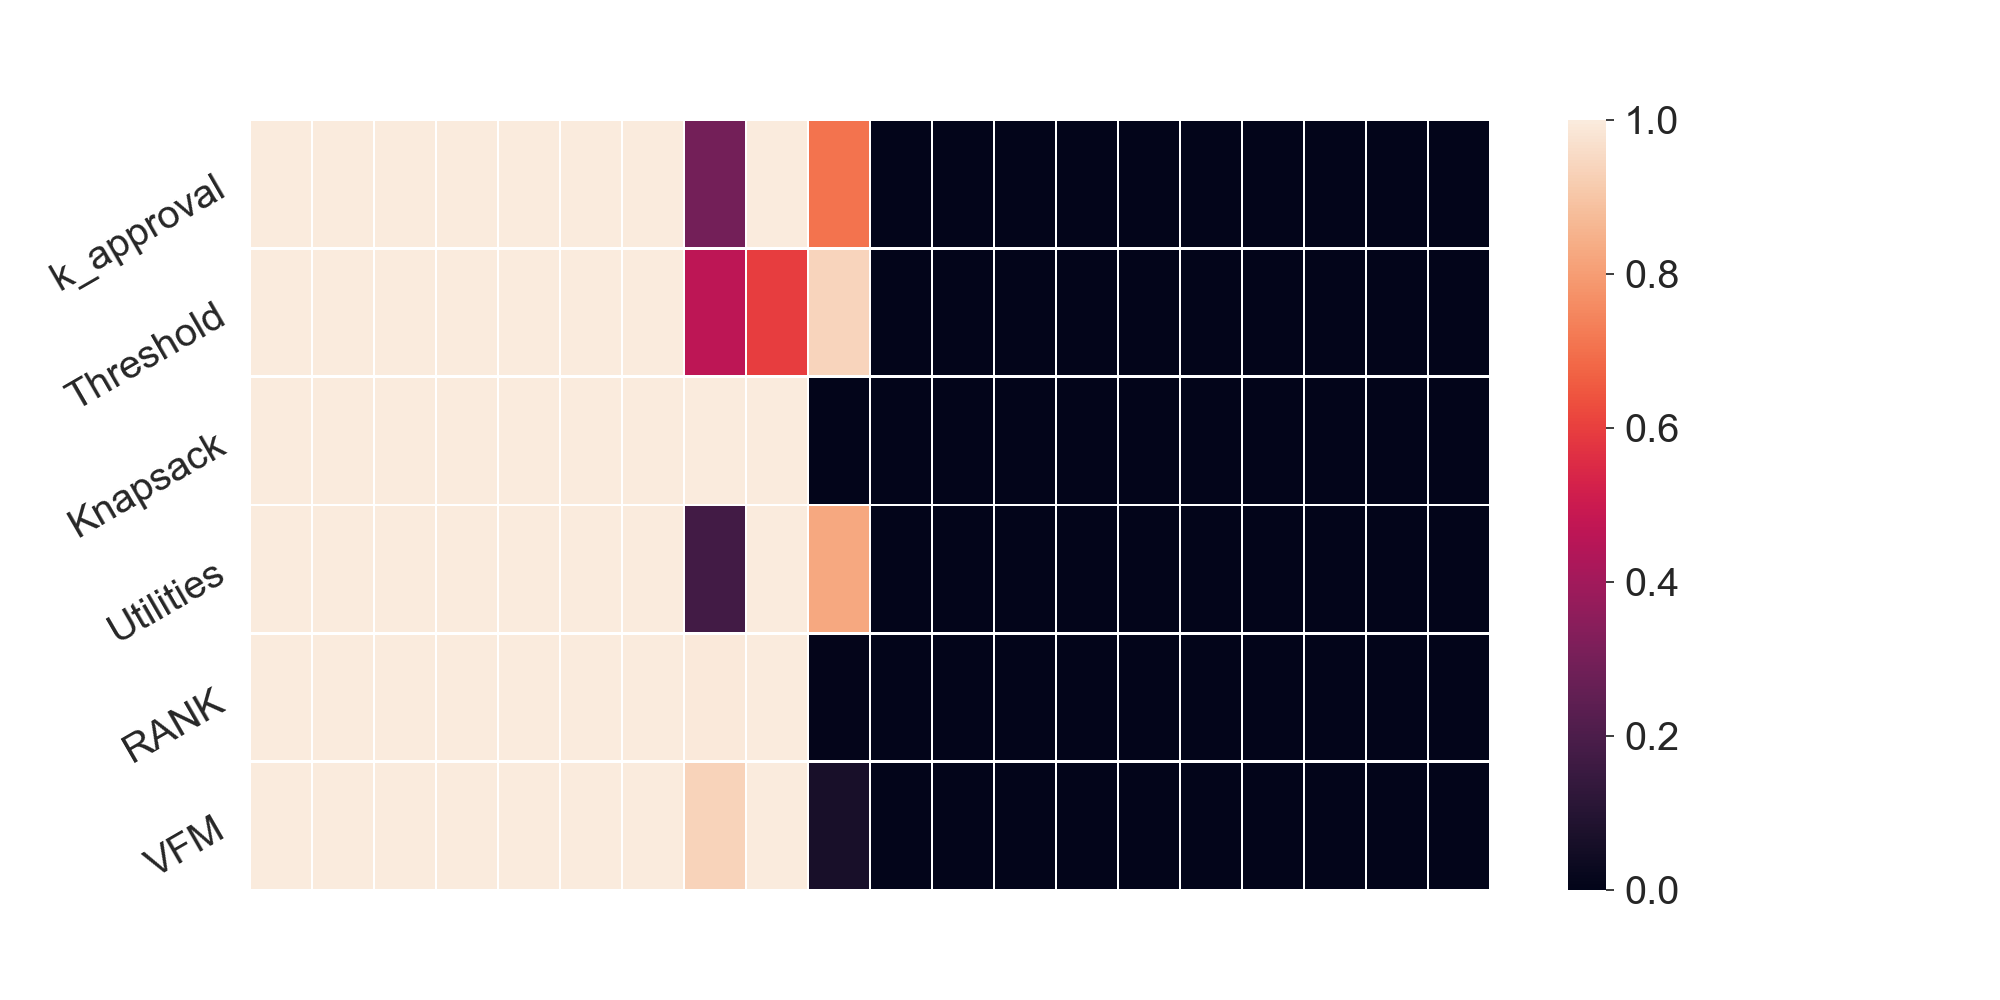
\includegraphics[width=18cm]{experiment/election_8_rx.png}
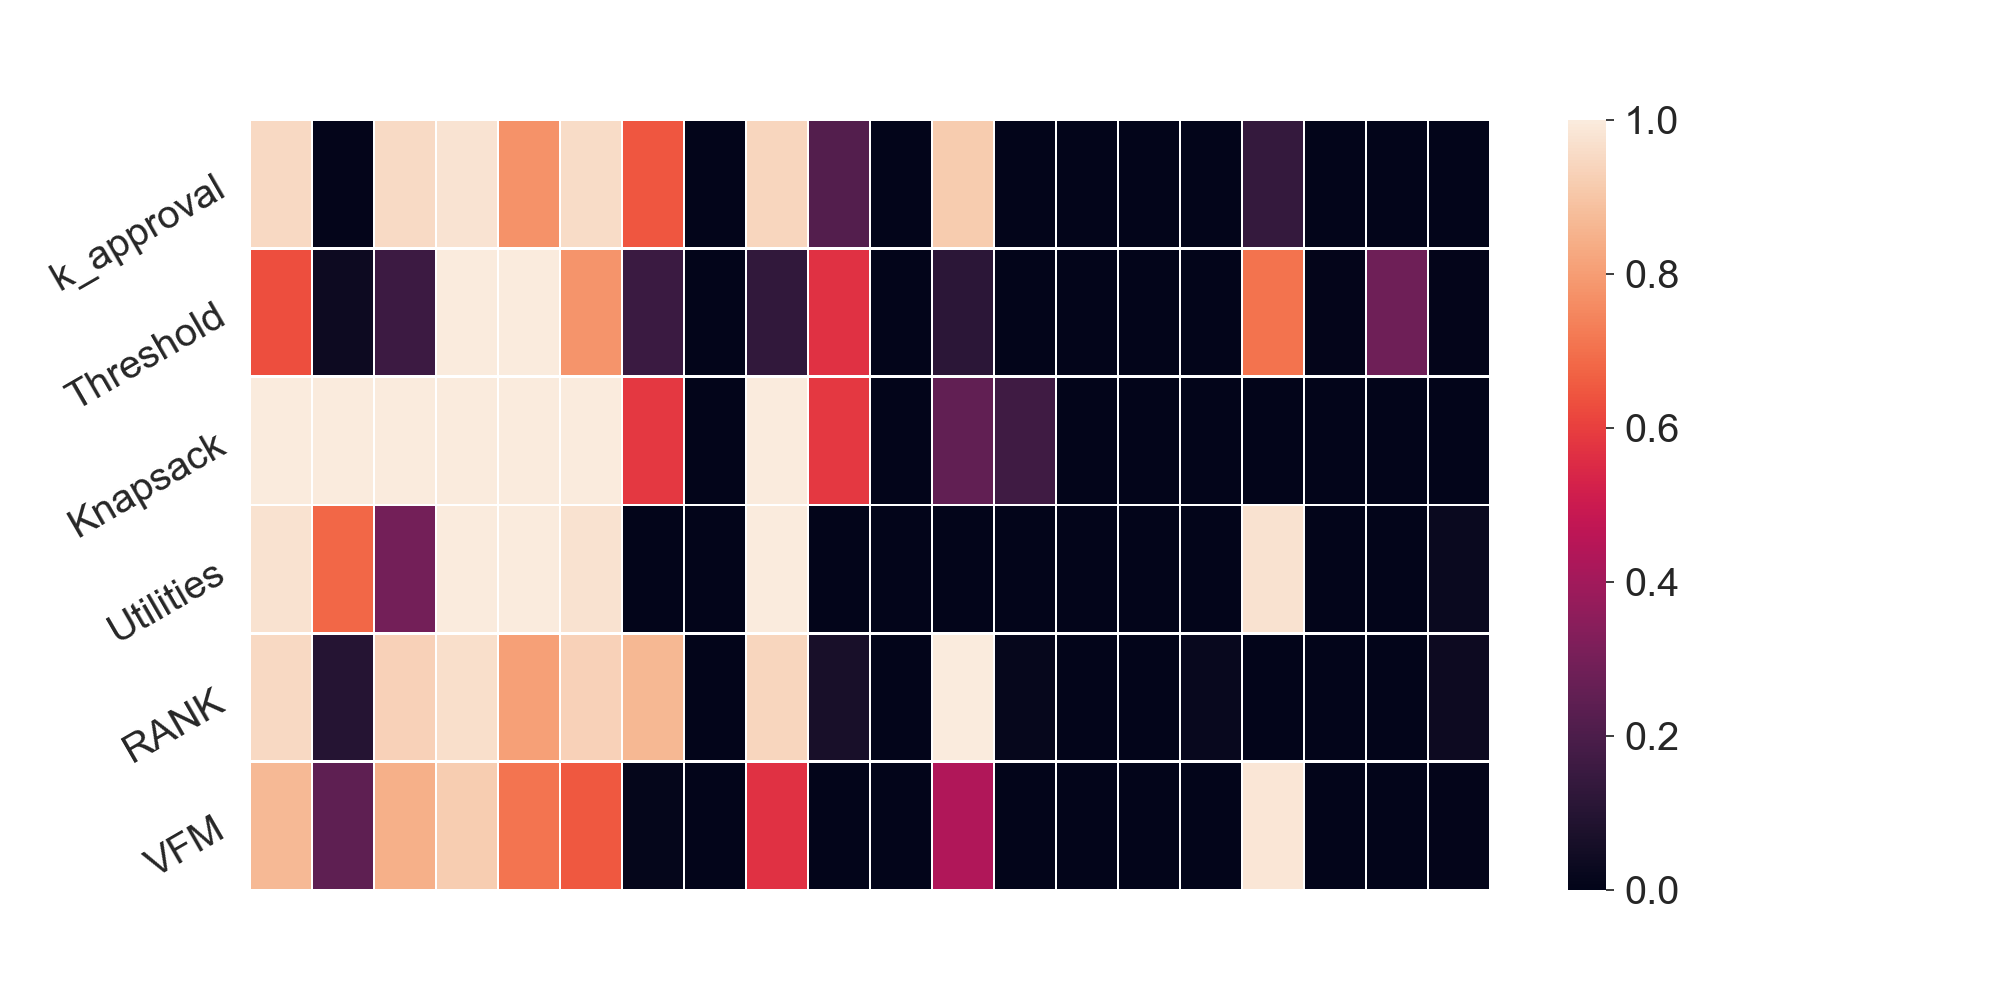
\includegraphics[width=18cm]{experiment/election_8_greedy.png}
\caption{Percentage of instances where each projects was selected for RX (top) and greedy (bottom)
aggregation for election 8.
}\label{fig:stability8}
\end{center}
\end{figure}



\end{appendices}


\end{document}
